%---------------------------------------------------------------------------%
%-                                                                         -%
%-                           LaTeX Template                                -%
%-                                                                         -%
%---------------------------------------------------------------------------%
%- Copyright (C) Huangrui Mo <huangrui.mo@gmail.com> 
%- This is free software: you can redistribute it and/or modify it
%- under the terms of the GNU General Public License as published by
%- the Free Software Foundation, either version 3 of the License, or
%- (at your option) any later version.
%---------------------------------------------------------------------------%
%->> Document class declaration
%---------------------------------------------------------------------------%
\documentclass[oneside]{Style/ucasthesis}%
%- Multiple optional arguments:
%- [<oneside|twoside|print>]% oneside eprint, twoside eprint, or paper print
%- [fontset=<adobe|...>]% specify font set to replace automatic detection
%- [plain]% thesis writing of international students
%- [draftversion]% show draft version information
%- [standard options for ctex book class: draft|paper size|font size|...]%
%---------------------------------------------------------------------------%
%->> Document settings
%---------------------------------------------------------------------------%
\usepackage[numbers,list]{Style/artratex}% document settings
%- usage: \usepackage[option1,option2,...,optionN]{artratex}
%- Multiple optional arguments:
%- [bibtex|biber]% set bibliography processor and package
%- [<numbers|super|authoryear|alpha>]% set citation and reference style
%- <numbers>: textual: Jones [1]; parenthetical: [1]
%- <super>: textual: Jones superscript [1]; parenthetical: superscript [1]
%- <authoryear>: textual: Jones (1995); parenthetical: (Jones, 1995)
%- <alpha>: textual: not available; parenthetical: [Jon95]
%- [geometry]% reconfigure page layout via geometry package
%- [lscape]% provide landscape layout environment
%- [xhf]% disable header and footer via fancyhdr package
%- [color]% provide color support via xcolor package
%- [background]% enable page background
%- [tikz]% provide complex diagrams via tikz package
%- [table]% provide complex tables via ctable package
%- [list]% provide enhanced list environments for algorithm and coding
%- [math]% enable some extra math packages
%- [xlink]% disable link colors
\usepackage{Style/artracom}% user defined commands
%---------------------------------------------------------------------------%
%->> Document inclusion
%---------------------------------------------------------------------------%
%\includeonly{Tex/Chap_1,...,Tex/Chap_N}% selected files compilation
%---------------------------------------------------------------------------%
%->> Document content
%---------------------------------------------------------------------------%
\lstset{
	language={[ANSI]C},
    numbers=left,numberstyle=\tiny,
	tabsize=2,
	frame=shadowbox
}
%-
%-> Titlepage information
%-
%---------------------------------------------------------------------------%
%->> Titlepage information
%---------------------------------------------------------------------------%
%-
%-> 中文封面信息
%-

\schoollogo[scale=2.5]{ucas_logo}% 校徽
\title{太湖之光并行计算开发入门}% 论文中文题目
\author{尹达恒}% 论文作者
\institute{江南大学超级计算俱乐部}% 机构名称
\date{2019年7月}% 毕业日期:夏季为6月、冬季为12月
%-
%-> 英文封面信息
%-
\TITLE{An Introduction to Parallel Programming on Sunway System}% 论文英文题目
\STATEMENT{Tutorial and tips for parallel programming beginners on Sunway \\ Based on porting and optimizing of mlpack}
\AUTHOR{Howard Yin}% 论文作者
\INSTITUTE{Supercomputer Club, Jiangnan University}% 院系名称
\DATE{July 2019}% 毕业日期:夏季为June、冬季为December
%---------------------------------------------------------------------------%
%
\begin{document}
%-
%-> Frontmatter: title page, abstract, content list, symbol list, preface
%-
\frontmatter% initialize the environment
%---------------------------------------------------------------------------%
%->> Frontmatter
%---------------------------------------------------------------------------%
%-
%-> 生成封面
%-
\maketitle% 生成中文封面
\MAKETITLE% 生成英文封面
%-
%-> 中文摘要
%-
\intobmk\chapter*{前\quad 言}% 显示在书签但不显示在目录
\setcounter{page}{1}% 开始页码
\pagenumbering{Roman}% 页码符号
\begin{itemize}
    \item 本书实际上是一个教程形式的学习笔记;
    \item 本书主要为不熟悉并行编程的同学编写,主要讲解具体的工具使用,不会过多涉及抽象的优化算法。玩过并行编程的同学请直接看超算中心发的两个手册,清华的大佬写的比我好,搞过CUDA写过cu玩过SIMD的一看就能懂;
    \item 本书主要的行文线索是2018年12月左右启动的机器学习算法库在太湖之光系统中的移植和并行优化项目;
    \item 本书是超算中心下发的官方教程《“神威 · 太湖之光”计算机编译系统用户手册 Version 0.9》(本书简称《编译手册》)和《神威 · 太湖之光并行程序设计与优化(第一版)Ver1.2》(本书简称《优化手册》)中重要知识点的实践总结;
    \item 比起Fortran作者更擅长也更常用C语言,C语言也能胜任超算系统中的大部分工作,因此本书所有代码均使用C语言编写,关于编译器也只涉及Sunway的C语言编译器;
    \item 本书不区分“‘神威 · 太湖之光’计算机系统”、“‘神威 · 太湖之光’系统”、“Sunway系统”、“神威系统”和“太湖之光系统”,以及处理器名称“SW26010”、“Sunway26010”和“申威26010”,请读者注意;
    \item 本书将作为每周的俱乐部工作报告持续更新。
\end{itemize}

\section*{学习本教程前需要掌握的知识}
\begin{itemize}
    \item C语言,不仅是C语言的使用,编译器的运行流程要了解。本书所有代码都是C语言,神威编译器也只介绍C语言编译器;
    \item 用命令行操作Linux系统(Sunway的操作系统没有图形界面);
    \item 看过某些并行计算教程开头的介绍章节(比如CUDA教程),至少知道并行计算是在干嘛。
\end{itemize}

\section*{国家超级计算中心简介}
神威·太湖之光超级计算机是由国家并行计算机工程技术研究中心研制、部署于国家超级计算无锡中心的超级计算机。类似的超级计算中心在国内共有7个,它们分别是:
\begin{itemize}
    \item 天津中心:2009年6月,滨海新区与国防科技大学签署合作协议共建国家超级计算天津中心。天津中心由国家科技部、滨海新区、开发区、国防科技大学共同投资6亿元建设,于2009年底开始投入运营。定位为国家重大科技服务平台、产业技术创新平台、人才聚集培养平台,主要承接国家“863”重大科技专项,是重要的大规模集成电路设计中心和基础软件工程中心及产业化基地;
    \item 深圳中心:国家超级计算深圳中心又称深圳云计算中心,总投资12.3亿元。主机系统由中国科学院计算技术研究所研制、曙光信息产业(北京)有限公司制造,2010年5月经世界超级计算机组织实测确认运算速度达每秒1271万亿次。深圳中心立足深圳、主要面向全国、服务华南、港、澳、台及东南亚地区,承担各种大规模科学计算和工程计算任务,同时以其强大的数据处理和存储能力为社会提供云计算服务;
    \item 长沙中心:国家超级计算长沙中心位于湖南大学校区内,其依托的计算设备是国防科技大学研制的“天河一号”超级计算机。长沙中心总投资7.2亿元,运算能力达每秒300万亿次,由湖南大学负责运营,国防科技大学提供计算设备和技术支持;
    \item 济南中心:国家超级计算济南中心主要依托的计算设备是“神威 · 蓝光”超级计算机,其持续性能可达0.796PFlops。济南中心秉持立足山东、辐射周边、服务全国的工作思路,积极服务于山东省"两区一圈一带"发展战略需求,支持国家重大科技创新和战略性新兴产业,服务地方经济发展。2018年8月,神威E级超算原型机在国家超级计算济南中心完成部署。
    \item 广州中心:国家超级计算广州中心由广东省人民政府、广州市人民政府、国防科技大学、中山大学共同建设,主要依托设备是“天河二号”超级计算机;
    \item 无锡中心:国家超级计算无锡中心是无锡市政府直属事业单位,由清华大学与无锡市政府共同建设,并委托清华大学管理运营。国家超级计算无锡中心依托的“神威 · 太湖之光”计算机系统是我国“十二五”期间“863计划”的重大科研成果,由国家并行计算机工程技术研究中心研制,运算系统全面采用了由国家高性能集成电路设计中心通过自主核心技术研制的国产“申威26010”众核处理器,是我国第一台全部采用国产处理器构建的世界排名第一的超级计算机;
    \item 郑州中心:2019年5月,国家超级计算郑州中心获得科技部批复筹建,成为全国第7家批复建设的国家超级计算中心,也是科技部出台认定管理办法后批复筹建的首家国家超级计算中心。郑州中心拟依托郑州大学建设运营,计划于2020年上半年建设完成,峰值计算能力预期将达到100Pflops。
\end{itemize}

\section*{神威 · 太湖之光简介}
“神威 · 太湖之光”计算机系统(Sunway TaihuLight)采用全机水冷、直流供电、高密度组装,配有精确的资源调度管理算法、丰富的并行编程语言和开发环境。2016年6月20日国际TOP500公布的排名数据中,“神威 · 太湖之光”计算机系统以每秒12.54亿亿次的峰值运算速度和9.3亿亿次的持续运算速度高居榜首。“神威 · 太湖之光”是中国第一台全部采用国内自主研发技术构建的超级计算机。详细的架构描述可见《优化手册》第一章。

\section*{申威26010简介}
“神威 · 太湖之光”计算机系统采用的处理器是申威26010(Sunway 26010),该处理器由上海高性能集成电路设计中心自主研制,其指令集为自主研发的64位申威指令集,工作频率1.5Ghz。该处理器不同于现有的纯CPU、CPU-MIC、CPU-GPU架构,而是采用了主-从核架构,每个申威26010中有4个处理器,每个处理器包含1个主核(运算控制核心)和64个从核(8x8核心阵列),主从核的关系类似于CPU-GPU架构。详细的架构描述可见《优化手册》1.2节。

\section*{同构计算和异构计算\cite{noauthor__nodate}}
同构计算是使用相同类型指令集和体系架构的计算单元组成系统的计算方式。同构超算只单纯使用一种处理器,例如“神威 · 蓝光”只采用了8704片申威1600。而异构计算主要是指使用不同类型指令集和体系架构的计算单元组成系统的计算方式。常见的计算单元类别包括CPU、GPU等协处理器、DSP、ASIC、FPGA等。例如天河2号有16000个计算节点,每个节点由2片Intel的E5 2692和3片Xeon PHI组成,共使用了32000片Intel的E5 2692和48000片Xeon PHI;天河1A使用了14336片Intel Xeon X5670处理器和7168片NVIDIA Tesla M2050高性能计算卡。相同功耗的情况下,异构超算能获得非常高的理论双精浮点性能和更高的性能功耗比,这也使异构处理器其更受超级计算机系统偏爱。

“神威 · 太湖之光”计算机系统所采用的申威26010属于异构众核处理器。不同于“神威 · 蓝光”的同构申威1600处理器和天河2号的CPU-GPU架构,申威26010的异构模式相当于将CPU和GPU集成在一个芯片上,从“神威 · 太湖之光”整体上看,这相当于将GPU分散放置到了CPU的周围,使得单个处理器同时具有CPU核GPU的功能。和CPU-GPU体系相比,这种架构的优势在于减少了计算过程中的数据传输时间,从而提高整体的运算速度。

%\keywords{中国科学院大学,学位论文,\LaTeX{}模板}% 中文关键词
%-
%-> 英文摘要
%-
%\intobmk\chapter*{Preface}% 显示在书签但不显示在目录

%前言 in English.

%\KEYWORDS{University of Chinese Academy of Sciences (UCAS), Thesis, \LaTeX{} Template}% 英文关键词
%---------------------------------------------------------------------------%
% title page, abstract
{% content list region
\linespread{1.2}% local line space
\intobmk*{\cleardoublepage}{\contentsname}% add link to bookmark
\tableofcontents% content catalog
}
%-
%-> Mainmatter
%-
\mainmatter% initialize the environment
%---------------------------------------------------------------------------%
%->> Main content
%---------------------------------------------------------------------------%
\chapter{Sunway系统的基本操作}\label{chap:introduction}

\section{登录}

未来Sunway官网和计算系统的登录方式可能变化,此处的登录方法仅供参考。超算中心下发了两套用户名和密码,一套用于登录VPN,一套用于登录SSH。

\subsection{登录Sunway系统SSL VPN}
\begin{enumerate}
    \item 使用IE浏览器\footnote{亲测Edge和Chrome在第一次登录时无法下载EasyConnect工具,卡在加载界面}进入神威·太湖之光官网www.nsccwx.cn;
    \item 在右上角“登录”处选择一个运营商进行登录(图\ref{fig:登录步骤1});
    \item 在弹出的警告页面\footnote{截至本章作成日2018年12月1日,太湖之光的官方网站服务器在使用自主生成的SSL证书进行https连接,这类非信任机构生成的证书会被现在的浏览器识别为不安全}中选择“详细信息”$\rightarrow$“转到此页面”(图\ref{fig:登录步骤2});
    \item 在登录界面输入俱乐部下发的VPN用户名密码进行登录(图\ref{fig:登录步骤3});
    \item 第一次登录完成后浏览器会自动下载EasyConnect工具,此工具为后续登录使用(图\ref{fig:登录步骤4}和图\ref{fig:登录步骤5})。
\end{enumerate}

再次登录时,打开第一次登录完成后自动下载的EasyConnect工具输入俱乐部下发的VPN用户名密码即可。

\subsection{SSH登录超算系统}
\begin{enumerate}
    \item 登录VPN;
    \item 在弹出的页面找到可用资源的IP地址(图\ref{fig:登录步骤6});
    \item 在命令行窗口输入“ssh [俱乐部下发的用户名]@[可用资源的IP地址]”命令进行登录\footnote{这里的用户名是SSH用户名},登录时会提示输入密码\footnote{多次登录有时会出现WARNING和登录失败,大部分情况下这都是神威系统为了安全对SSH登录验证的公钥进行定时修改所致(猜测)。这时只要删除用户目录下的C:/用户/用户名/.ssh/known\_hosts文件重新登录SSH即可(这个文件记录了所有登录过的SSH服务器的公钥,再次登录时会进行公钥比对,如果不符则登录失败)},此处密码为SSH登录密码(图\ref{fig:登录步骤7});
    \item 出现bash界面说明登录成功(图\ref{fig:登录步骤8})。
\end{enumerate}

\begin{figure}[!htbp]
    \centering
    \begin{subfigure}[b]{0.49\textwidth}
      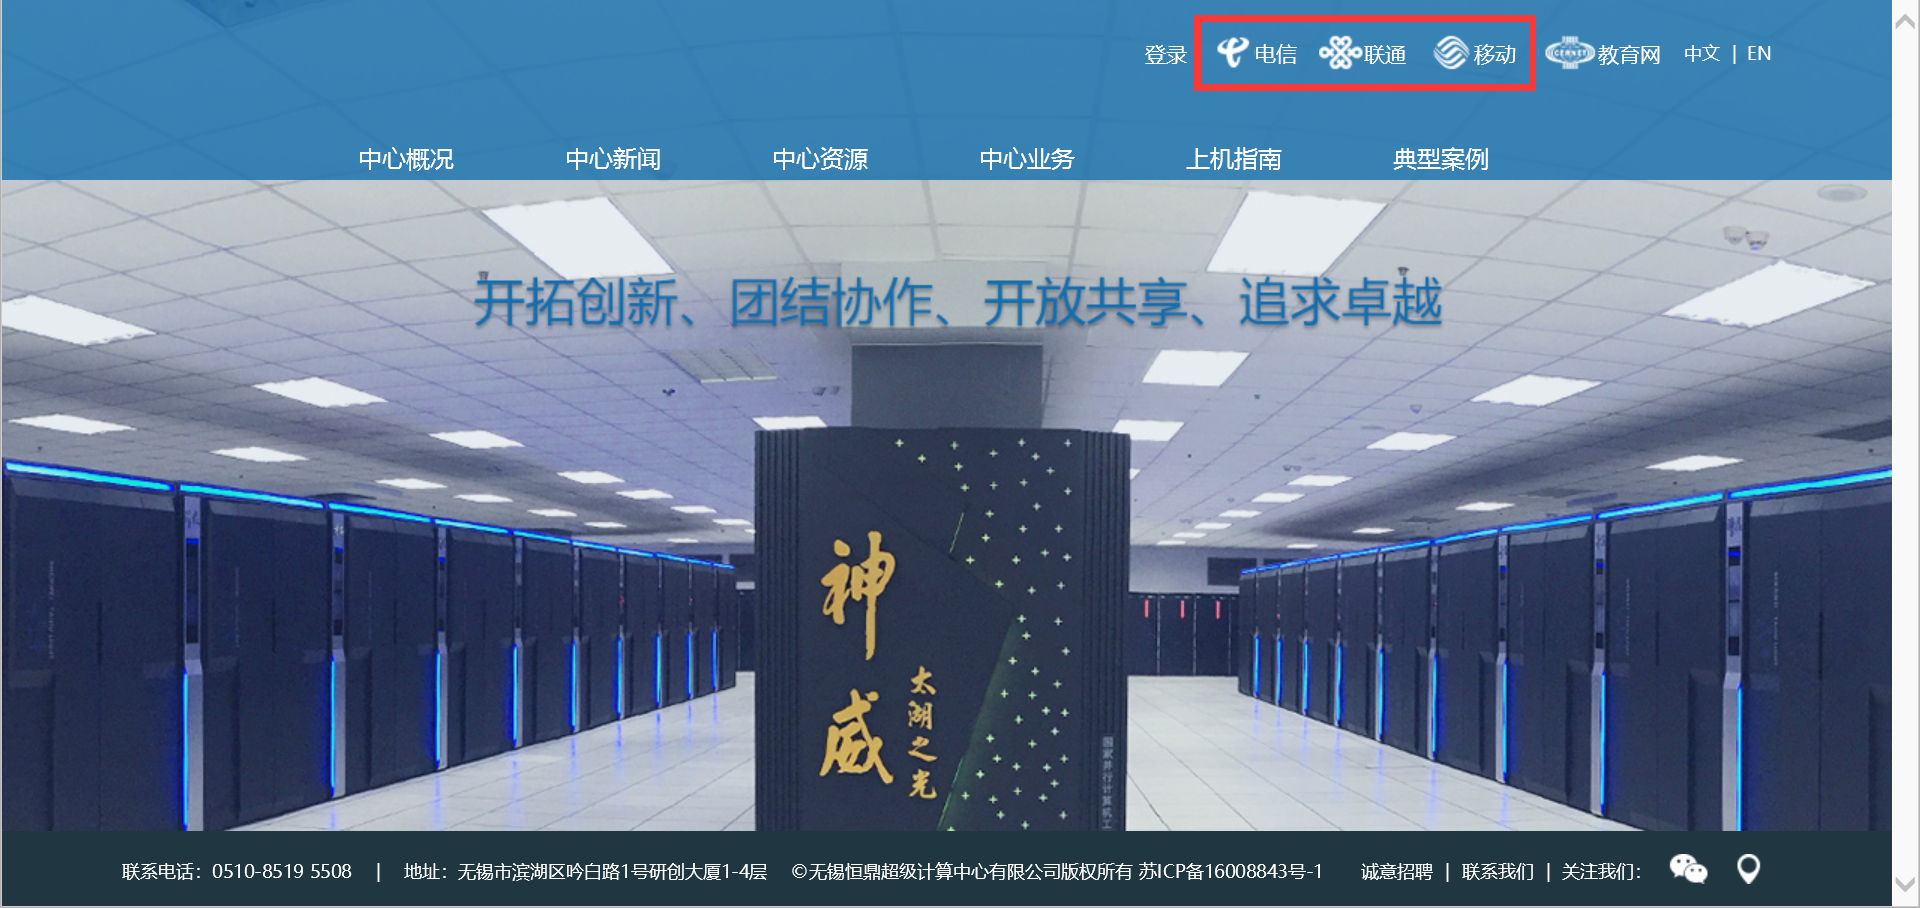
\includegraphics[width=\textwidth]{Login/1.png}
      \caption{官网主页}
      \label{fig:登录步骤1}
    \end{subfigure}%
    ~% add desired spacing
    \begin{subfigure}[b]{0.49\textwidth}
      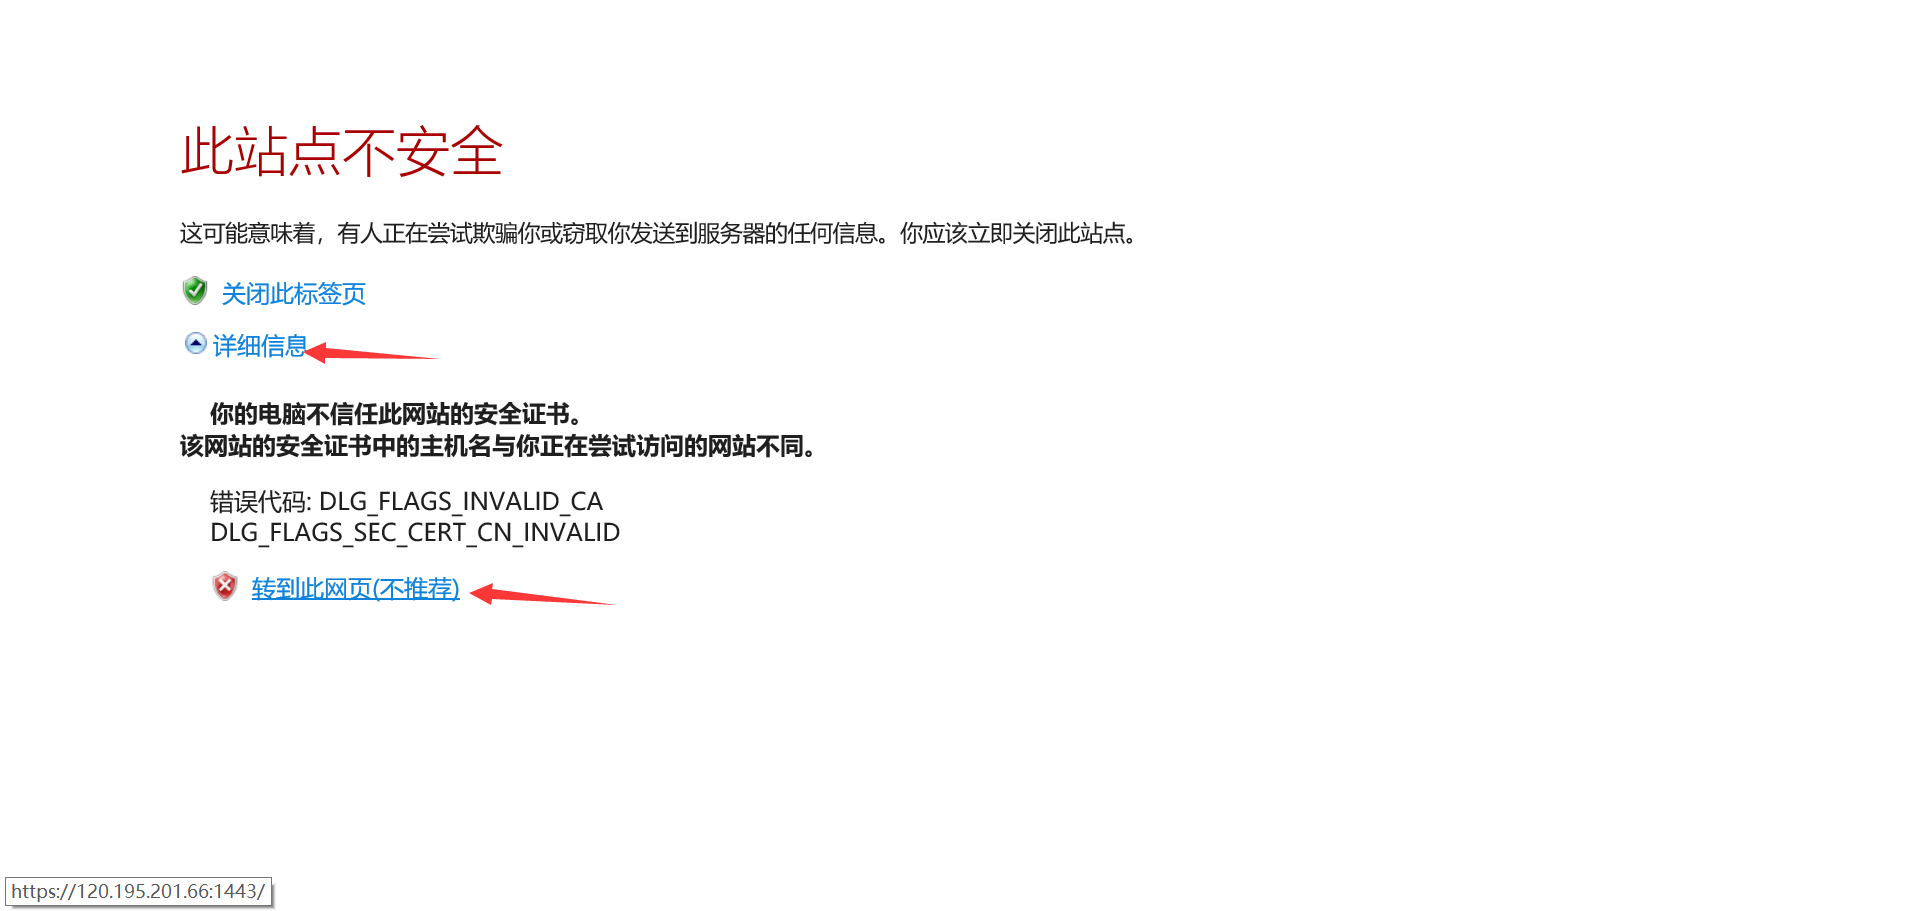
\includegraphics[width=\textwidth]{Login/2.png}
      \caption{进入登录页面}
      \label{fig:登录步骤2}
    \end{subfigure}
    \\% line break
    \begin{subfigure}[b]{0.49\textwidth}
      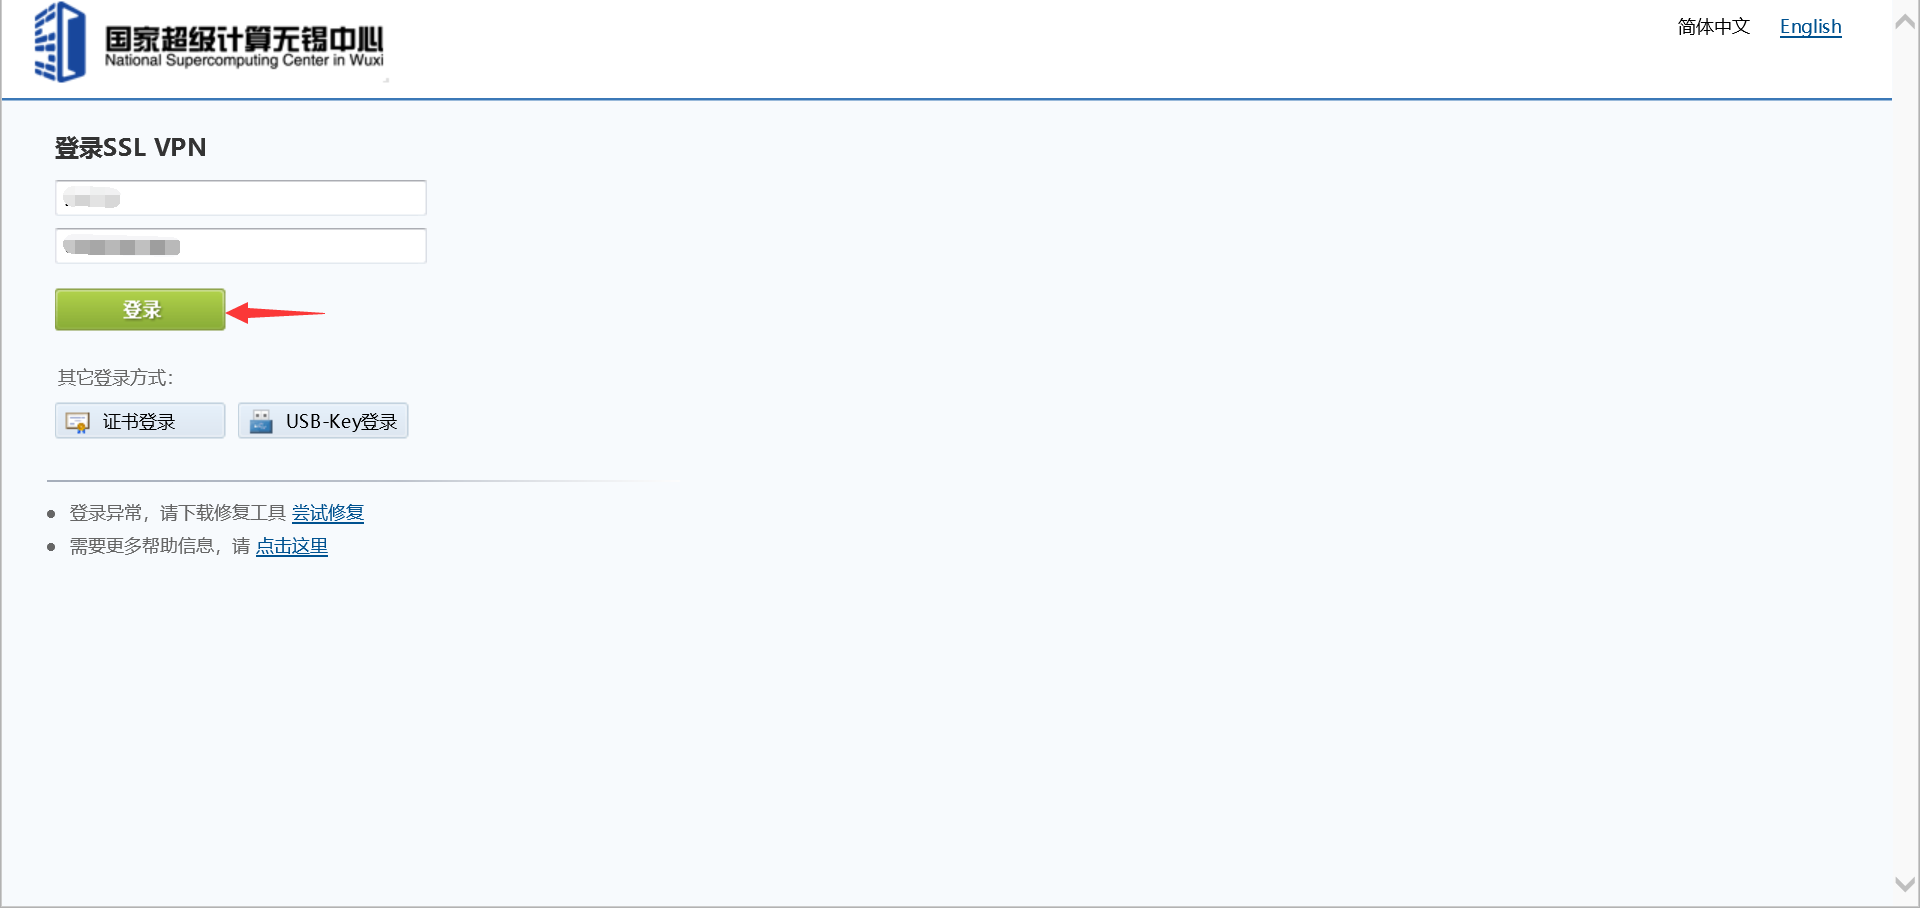
\includegraphics[width=\textwidth]{Login/3.png}
      \caption{登录VPN}
      \label{fig:登录步骤3}
    \end{subfigure}%
    ~% add desired spacing
    \begin{subfigure}[b]{0.49\textwidth}
      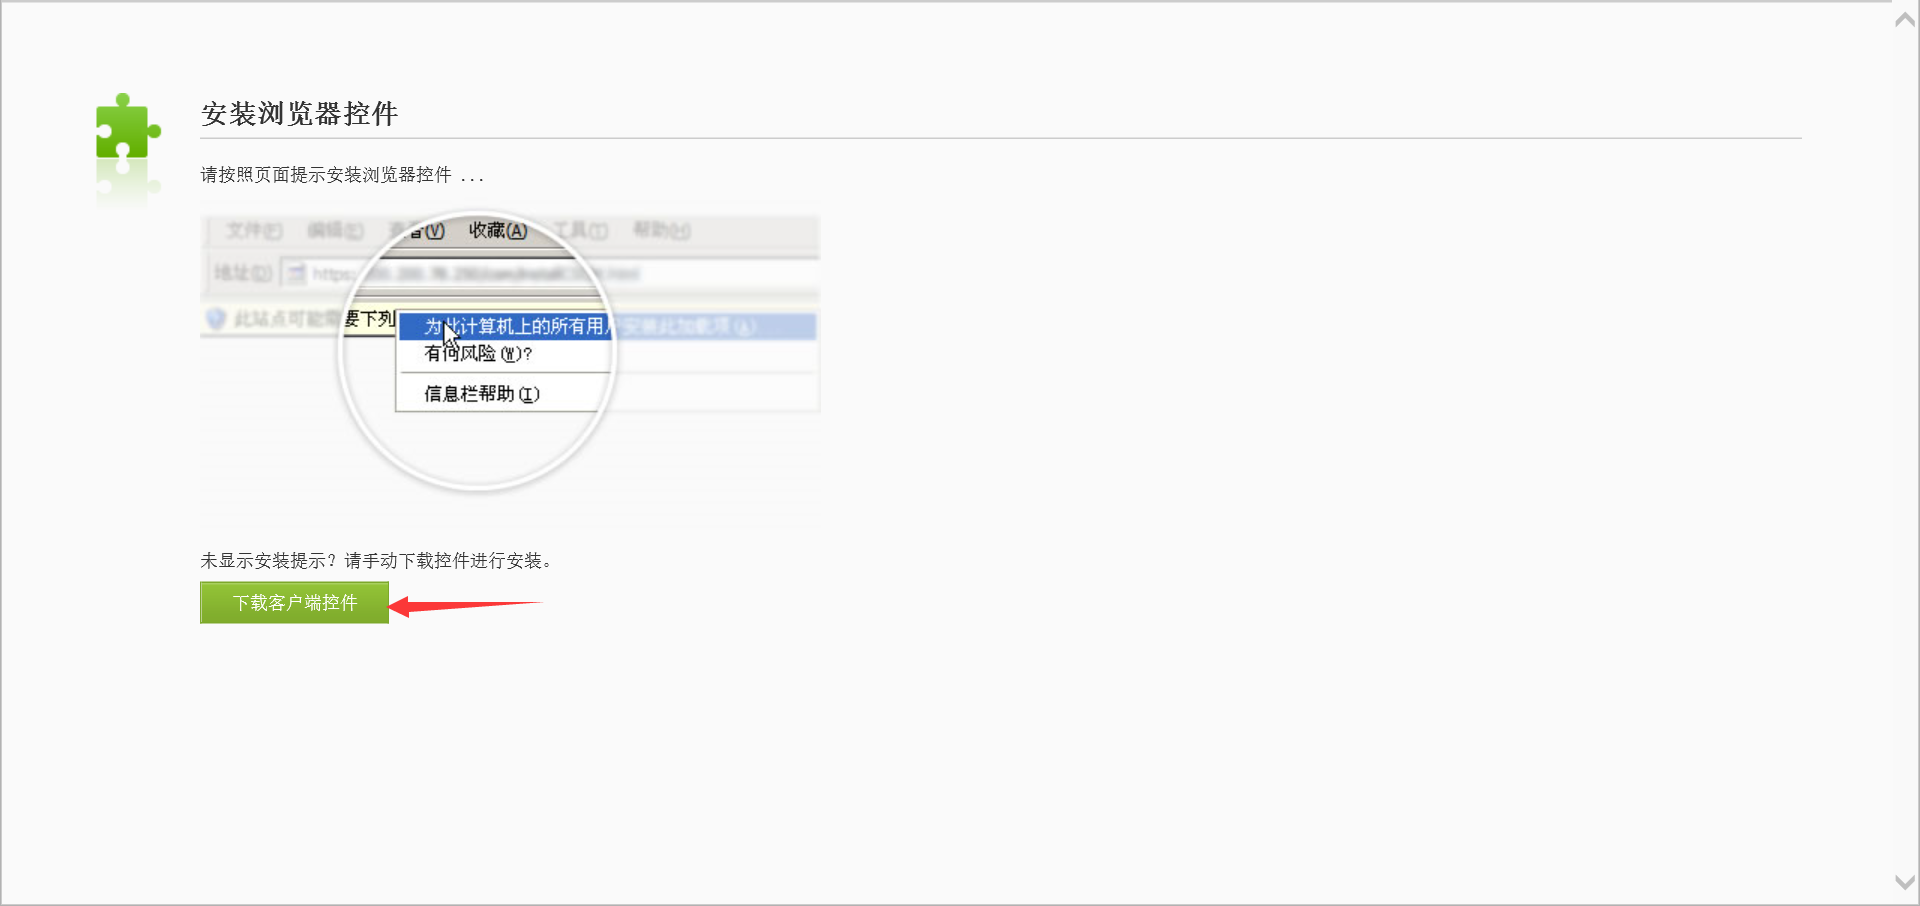
\includegraphics[width=\textwidth]{Login/4.png}
      \caption{下载EasyConnect}
      \label{fig:登录步骤4}
    \end{subfigure}
    \\% line break
    \begin{subfigure}[b]{0.49\textwidth}
      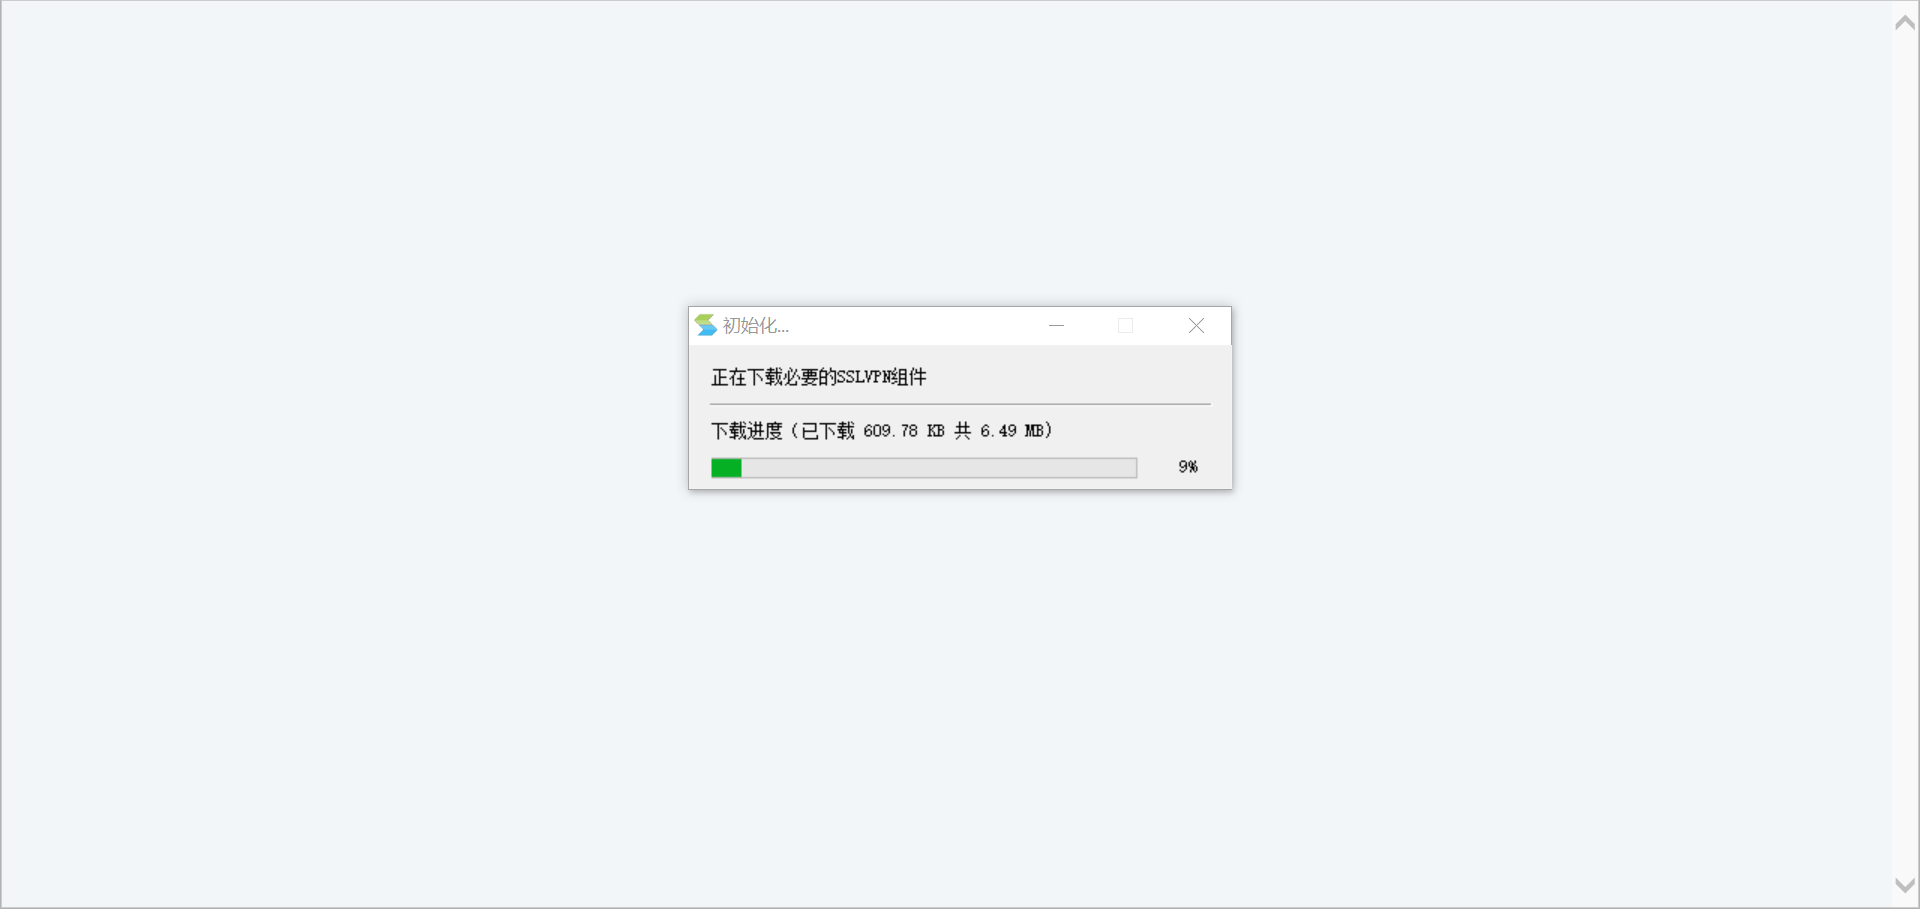
\includegraphics[width=\textwidth]{Login/5.png}
      \caption{安装EasyConnect}
      \label{fig:登录步骤5}
    \end{subfigure}%
    ~% add desired spacing
    \begin{subfigure}[b]{0.49\textwidth}
      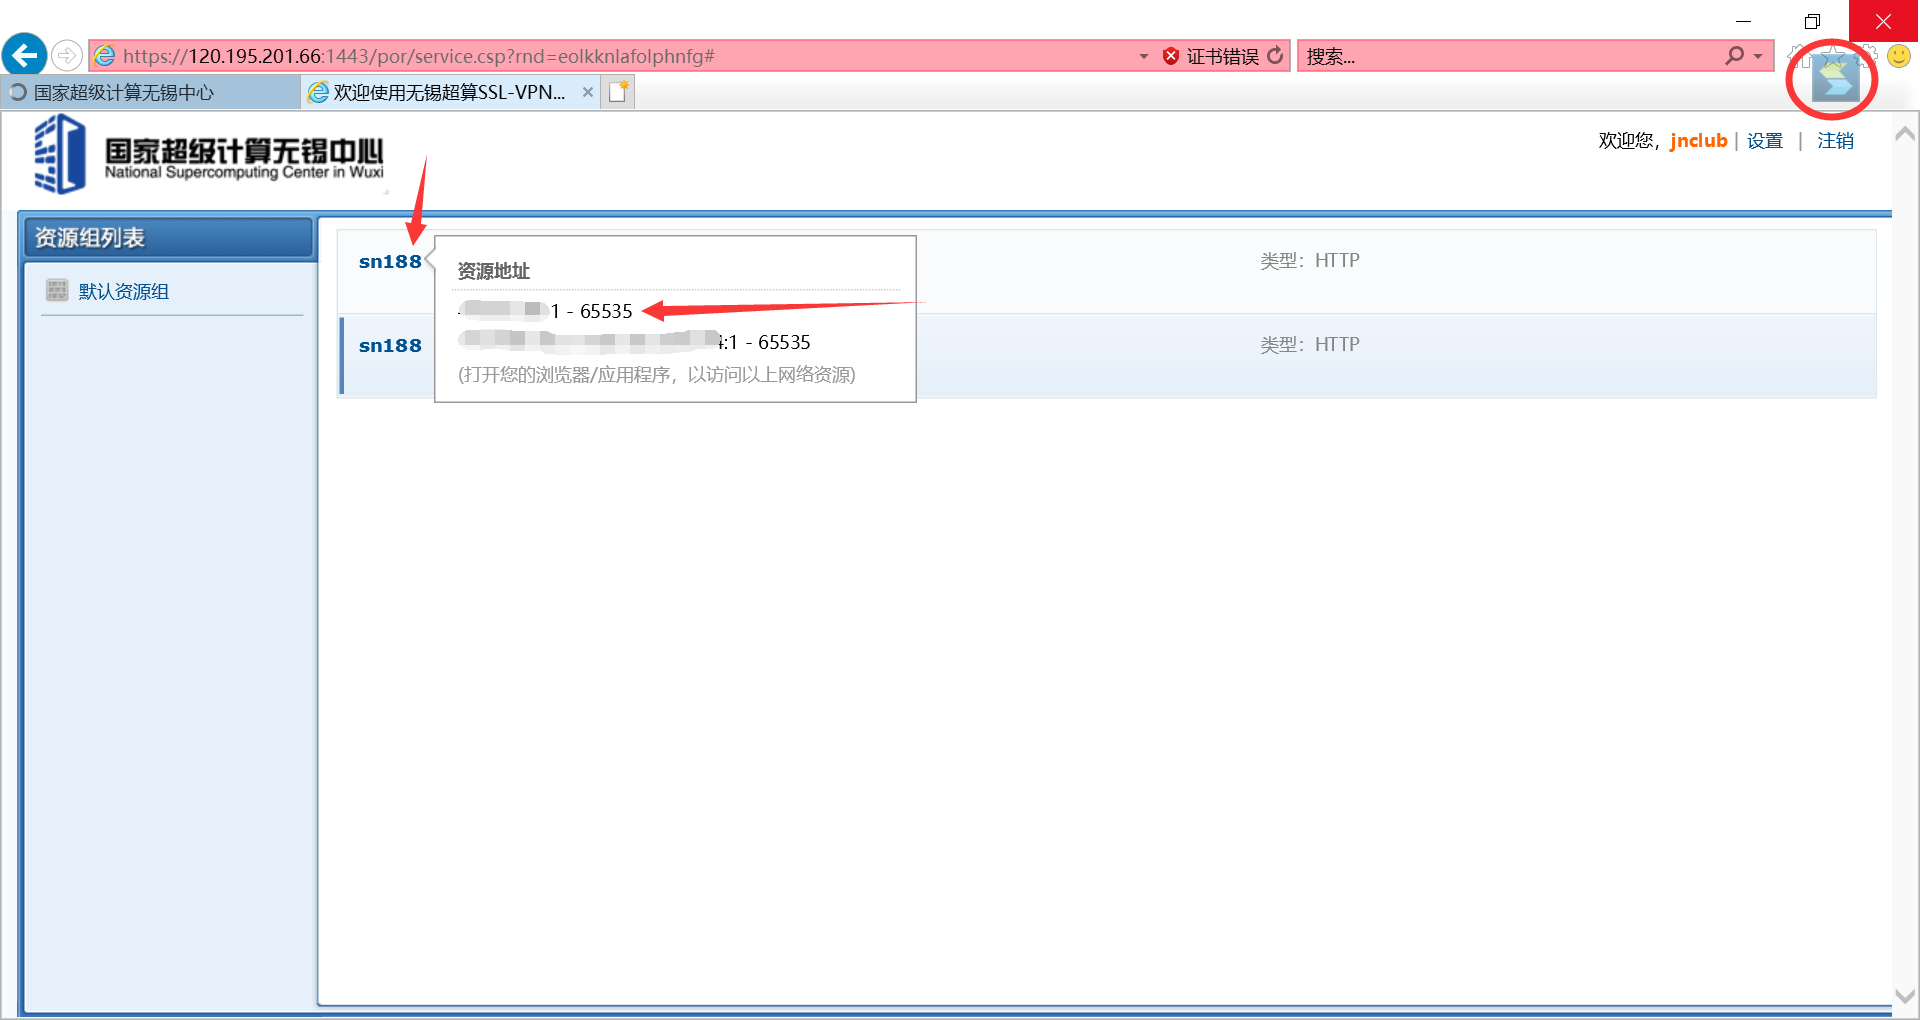
\includegraphics[width=\textwidth]{Login/6.png}
      \caption{找可用资源}
      \label{fig:登录步骤6}
    \end{subfigure}
    \\% line break
    \begin{subfigure}[b]{0.49\textwidth}
      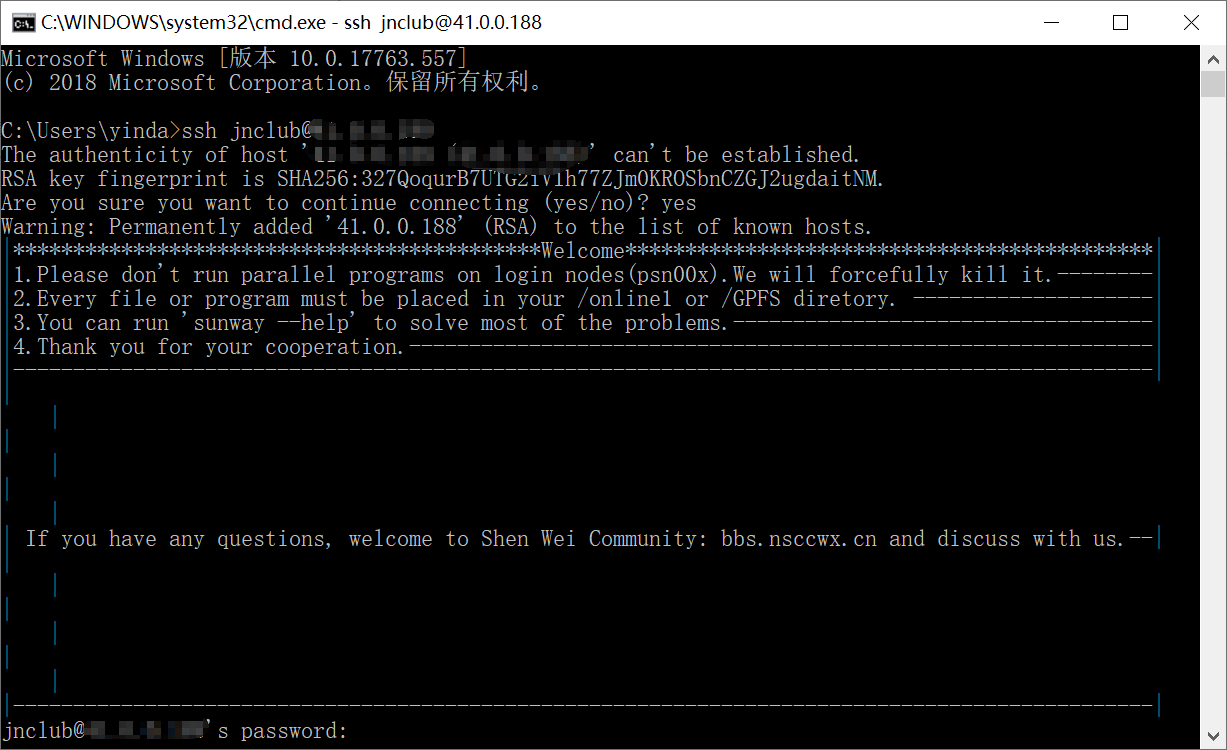
\includegraphics[width=\textwidth]{Login/7.png}
      \caption{用可用资源IP登录SSH}
      \label{fig:登录步骤7}
    \end{subfigure}%
    ~% add desired spacing
    \begin{subfigure}[b]{0.49\textwidth}
      
\includegraphics[width=\textwidth]{Login/8.png}
      \caption{登录成功}
      \label{fig:登录步骤8}
    \end{subfigure}
    \caption{超算系统登录流程}
    \label{fig:oaspl}
\end{figure}

\section{第一个程序:矩阵相加}
矩阵计算是所有并行计算的基础,第一个并行程序以矩阵相加程序为例,介绍在单个SW26010处理器上编程时Sunway编译器和Athread的一些基本操作。矩阵相加程序的要求非常简单:将两个64x2048的矩阵相加。

\subsection{单个SW26010处理器并行计算流程}\label{section:并行计算的基本流程}
正如前言中所说,每个SW26010芯片中都包含4个处理器,每个处理器有1个主核和64个从核,第一个程序的编写将着眼于在一个处理器上的编程,程序只使用1个主核和64个从核。

\begin{enumerate}
	\item 运行于主核上的主程序启动N个并行执行的线程(N$\leq$64),每个线程都在一个从核上执行;
	\item 在并行执行的线程中,每个线程都从主存储中\textbf{不同的位置}取出数据放入从核各自的局部存储中\footnote{在一般的并行编程中都有在并行线程中获取线程编号的方法,并行线程即通过线程编号计算出自己要从哪个位置取数\label{footnote:取数据说明}}\footnote{从主存储中取出数据放入从核的局部存储使用称作DMA(Direct Memory Access,直接内存存取)的方法,DMA运行独立于主核和从核,可以在主核和从核进行计算的同时传输数据,在基于传输的并行优化方面尤其有用\label{footnote:DMA}};
	\item 从核在自己的局部存储上进行计算;
	\item 从核计算完成后,都分别将计算结果放回到主存储中后结束自身的线程;
	\item 在从核运行过程中主程序进行其他其他操作并等待所有从核线程结束;
	\item 所有的从核线程结束(从核函数退出)之后,主程序进行下一步并行操作或结束。
\end{enumerate}

\subsection{相关Athread函数}
下面是矩阵相加程序中使用到的并行函数相关必要知识的介绍,更加详细的描述见《编译手册》第五章“加速线程库”。
\subsubsection{在主核中调用的Athread函数}
\begin{enumerate}
	\item athread\_init()核组初始化,在所有athread操作之前都要进行调用;
	\item athread\_set\_num\_threads()设置下一次并行操作启动的线程总数,如果不设置此项值则下一次并行操作(athread\_spawn)启动64个线程;
	\item athread\_spawn([函数指针],[传入参数])在从核上启动并行线程,[函数指针]为指向从核函数入口的指针(从核函数名),且该指针需要在文件开头使用一个Athread库中的宏“extern SLAVE\_FUN(从核函数名)()”进行声明;[传入参数]为向每个从核函数传递的实参该参数会在运行时传递到每个并行从核函数线程中;
	\item athread\_join()等待所有从核线程结束,程序执行到此函数时会阻塞直到所有从核线程结束才会执行下一步;
	\item athread\_halt()关闭线程组流水线,在所有并行操作完成之后才能调用此函数,在程序结束时调用,调用后运算核心将无法在本进程中再次使用。
\end{enumerate}

\subsubsection{在从核中调用的Athread函数}
\begin{enumerate}
	\item athread\_get\_id()获取线程逻辑标号,一般在从核程序中通过此函数的值判断应该从主存储的哪个位置取数据;
	\item athread\_get([传输模式],[源地址],[目的地址],[数据量],[回答字地址],[],[],[])通过DMA(见注\ref{footnote:DMA})方法从主存中读取数据写入从核局部存储。各形参含义为:
	\begin{itemize}
		\item 传输模式:DMA传输命令模式,本例程中只涉及使用PE\_MODE;
        \item 源地址:要传输的数据在主核中的地址(在主核程序中的变量名)。对于数组形式的数据,此处填数组变量的首地址,就像下面这样\footnote{这里的取数位置即是从核函数要从何处取数的标志(见注\ref{footnote:取数据说明}),该值一般由athread\_get\_id()获取到的线程逻辑标号计算得出}。多维数组的取址方法以此类推。
		\begin{lstlisting}
&源数组名[取数位置]//一维数组首地址位置
&源数组名[取数位置1][取数位置2]//二维数组首地址位置
        \end{lstlisting}
        上面写出的源数组名数组名需要在从核程序开头进行“extern”声明,如下所示。
		\begin{lstlisting}
extern 数据类型 源数组名;//文件开头声明主核中的某个数组
		\end{lstlisting}
		\item 目的地址:从主存中取得的数据放入局部存储的哪个地址(变量)中。对于数组形式的数据其写法和源地址相同,且数组名需要在从核函数文件开头进行“\_\_thread\_local”声明,如下所示。
		\begin{lstlisting}
extern 数据类型 源数组名;//文件开头声明主核中的某个数组
		\end{lstlisting}
		\item 数据量:从源地址开始读取多少\textbf{字节}数据到局部存储(目的地址)中。对于数组形式的数据,此参数的值为[要读多少个数]*[此数组的数据类型占多少字节]\footnote{实测在太湖之光的编译系统中,int型和float型占4个字节,long型和double型占8个字节}。
		\item 回答字地址:当athread\_get数据传输完成时,回答字地址中的值加1。多个athread\_get同时运行可以共用一个回答字,每个athread\_get运行结束时都会使回答字地址中的值加1。一般在等待athread\_get传输完成的地方会有“while([回答字]!=[共用此回答字的athread\_get函数个数]);”。回答字变量在从核函数文件开头以“\_\_thread\_local volatile”声明。
		\item 本例程不涉及最后三个参数。
	\end{itemize}
\end{enumerate}


\subsection{并行编程思路}\label{subsec:并行编程思路}
并行编程程序分主核和从核两个程序流程,请理解上文所述的各函数的作用并理解下列流程后自行编写程序。参考程序见附录\ref{apdx:第一个程序}。
\newline 主核程序:
\begin{enumerate}
    \item 生成两个64x2048矩阵;
    \item athread\_init()初始化;
    \item athread\_spawn()启动64个从核线程,每个线程处理每个64X2048矩阵中的2048个数;
    \item athread\_join()等待线程全部结束;
    \item athread\_halt()关闭线程流水线;
    \item 输出结果,退出程序。
\end{enumerate}
从核程序:
\begin{enumerate}
    \item athread\_get\_id()获取线程逻辑标号;
    \item athread\_get()根据线程逻辑标号从主核程序变量中取得要用的数据,每个线程取在两个64x2048矩阵中各取2048个数;
    \item 计算相加结果;
    \item athread\_put()将结果写回主核程序变量中;
    \item 退出程序。
\end{enumerate}

\section{程序的编译}
“神威 · 太湖之光”系统的编译环境有两种,一种是服务于高速计算系统的编译环境,即SW26010搭建的神威主系统;另一种服务于辅助计算系统,该系统是常见的Intel X86 CPU + GPU结构服务器。这里只介绍高速计算系统环境下的程序编译。本节主要内容来自《优化手册》2.5节“编译环境”。

\subsection{Sunway程序编译简介}
目前的“神威 · 太湖之光”系统支持的编程语言主要包括C语言(C99)、C++语言(C++03和C++11)和Fortran(Fortran2003),其中C++目前还不能编译从核程序。

神威系统的C语言编译器指令为“sw5cc”,编译模式分为主核和从核两种\footnote{正如前言中所说,异构计算使用不同类型指令集和体系架构的计算单元组成系统,因此在编译程序时主核和从核使用的编译器并不相同},编译主核程序的指令为:
\begin{lstlisting}
sw5cc -host [选项] 文件名.c
\end{lstlisting}
编译从核的指令为:
\begin{lstlisting}
sw5cc -slave [选项] 文件名.c
\end{lstlisting}
主核程序和从核程序编译完成后,则使用下面这个命令进行混合链接生成可执行程序:
\begin{lstlisting}
sw5cc -hybrid [选项] 主核文件名.o 从核文件名.o
\end{lstlisting}

本章只介绍编译器的基本使用方法,不过多涉及编译器的编译选项,详细了解编译选项可见《优化手册》表格2-2。

\subsection{用命令行编译程序}\label{subsec:用命令行编译程序}
假设在\ref{subsec:并行编程思路}节编写的主核程序源文件名“master\_arrAdd.c”、从核程序源文件名“slave\_arrAdd.c”,则可以输入下面这三条指令对源文件进行编译和链接:
\begin{enumerate}
  \item 编译主核,-c选项表示为每个源文件生成一个.o文件但不进行链接
\begin{lstlisting}
sw5cc -host -c master_arrAdd.c
\end{lstlisting}
  \item 编译从核
\begin{lstlisting}
sw5cc -slave -c slave_arrAdd.c
\end{lstlisting}
  \item 链接,-o arrAdd选项表示输出的可执行文件名为“arrAdd”
\begin{lstlisting}
sw5cc -hybrid master_arrAdd.o slave_arrAdd.o -o arrAdd
\end{lstlisting}
\end{enumerate}

编译完成后即可在当前目录下看到一个可执行文件“arrAdd”。接下来介绍运行这个可执行文件的方法。

\section{程序的运行}
和上一节介绍的编译环境一样,神威系统的运行也分高速计算系统运行和辅助计算系统运行两种,这里也只介绍程序在高速计算系统中的运行,主要内容来自《优化手册》2.6节“作业提交”。

\subsection{Sunway程序运行简介}
“神威 · 太湖之光”的高速计算系统计算资源由一个作业管理系统进行管理,其本质是一个队列。在高速计算系统上运行的程序称为“作业”,要运行某个作业时,将这个作业提交到作业管理系统的队列中,作业管理系统按照先进先出方式取出队列中的作业放到计算节点上运行。

俱乐部目前持有的账号可以向免费的开发调试计算队列提交作业:高速计算系统的q\_sw\_expr和辅助计算系统的q\_x86\_expr。这两个队列中每个作业的最长运行时间为60分钟,最大并行规模为64。

\subsection{用命令行运行程序}
神威系统提交作业的指令为“bsub”,其指令选项内容丰富,此处不一一展开,详细的选项可见《优化手册》2.6.2节,这里只介绍几个常见的选项。

使用“bsub”指令运行\ref{subsec:用命令行编译程序}中编译完成的可执行程序“arrAdd”,可键入如下指令:
\begin{lstlisting}
bsub -I -b -q q_sw_expr -n 1 -cgsp 64 ./arrAdd
\end{lstlisting}
指令选项解释:
\begin{itemize}
  \item -I:使作业输出在当前窗口;
  \item -q q\_sw\_expr:将作业提交到q\_sw\_expr计算队列;
  \item -b:指定从核栈位于局部存储,该选项使得从核程序先全部读入从核局部再运行,可以减少主从核数据传输的次数,对于并行计算的速度提升非常重要;
  \item -n 1:指定程序要用的核组个数为1;
  \item -cgsp 64:指定每个核组内要用的从核个数为64,由于一个SW26010一个核组只有64个从核,因此该值不能大于64。该选项即影响程序中athread\_spawn()生成的从核线程的个数;
  \item ./arrAdd:要执行的可执行文件位置。
\end{itemize}

若使用附录\ref{apdx:第一个程序}中的程序,在程序执行完成后可得到并行和非并行计算的结果与时间对比。

\section{总结}
\subsection{知识点概括}
本章主要介绍了在神威系统编写程序的流程和必须要知道的一些基本操作,内容可大致概括为图\ref{fig:Chap_Intro}。

\begin{figure}[!htbp]
  \centering
  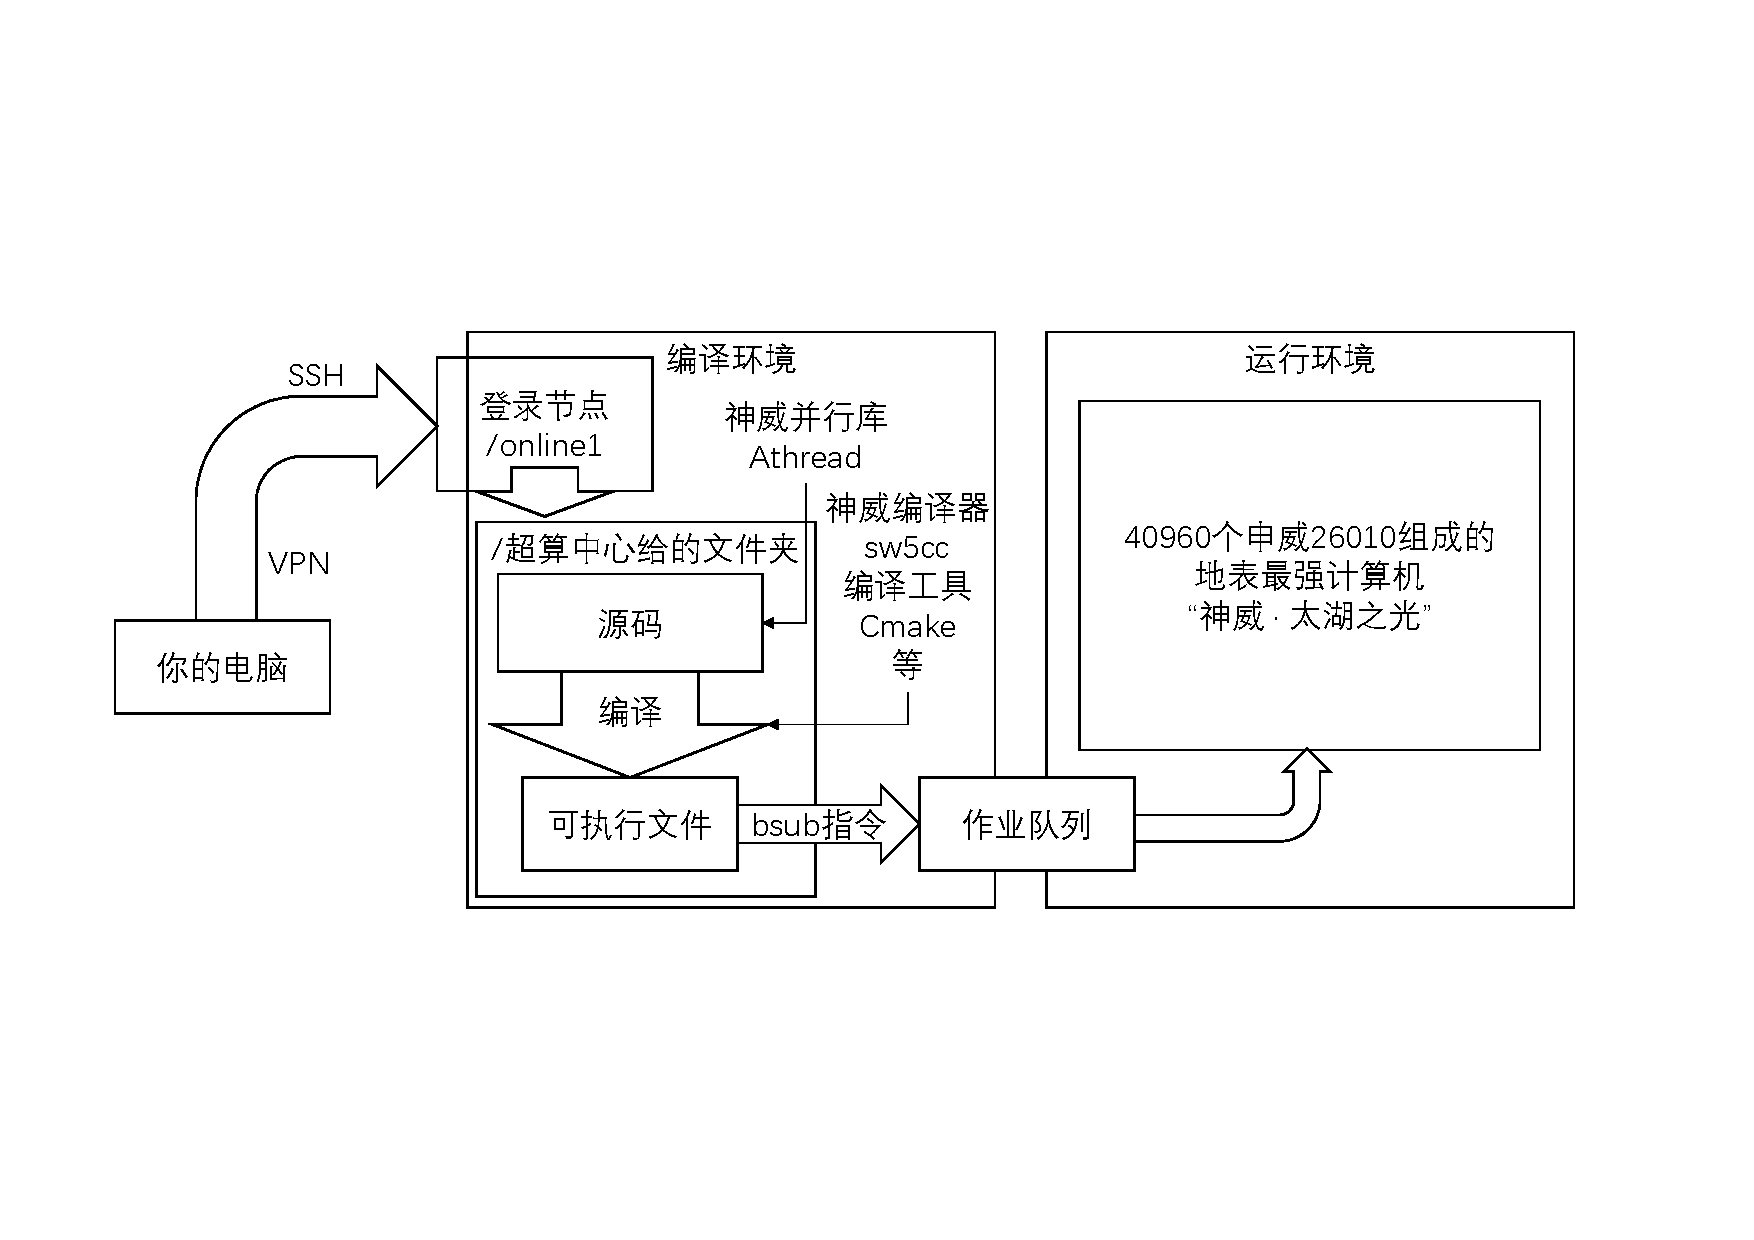
\includegraphics[width=\textwidth]{Chap_Intro}
  \caption{第一章的知识点概括}
  \label{fig:Chap_Intro}
\end{figure}

\subsection{练习}
\begin{itemize}
  \item 用Athread实现并行的矩阵减法;
  \item 用Athread实现并行的矩阵乘法。
\end{itemize}
\chapter{Darknet移植}
\section{Darknet介绍}
Darknet是一个开源的C语言神经网络框架,由著名的机器视觉专家Joseph Redmon开发\cite{darknet13}。Darknet性能优异,安装简单,在目标识别领域有广泛应用的YOLO模型\cite{yolov3}的最初版本就是在这个框架下开发的。作为作为“神威 · 太湖之光”并行编程的入门练习,Darknet有如下优点\cite{darknet_note}:
\begin{itemize}
    \item 易于安装:在makefile里面选择自己需要的附加项(cuda,cudnn,opencv等)直接make即可;
    \item 没有任何依赖项:整个框架都用C语言进行编写,可以不依赖任何库,连opencv作者都编写了可以对其进行替代的函数;
    \item 结构清晰:其框架的基础文件都在src文件夹,而定义的一些检测、分类函数则在example文件夹,可根据需要直接对源代码进行查看和修改;
    \item 友好python接口:虽然darknet使用c语言进行编写,但是也提供了python的接口,通过python函数,能够使用python直接对训练好的.weight格式的模型进行调用;
    \item 易于移植:该框架部署十分简单,且可以根据机器情况,使用cpu和gpu,特别是检测识别任务的本地端部署,darknet会显得异常方便。
\end{itemize}

此外,由于Darknet是一个神经网络框架,其中的主要运算任务都可以以矩阵计算的形式所表述,这使得Darknet的移植和优化有助于读者对矩阵和并行更加深入的理解。最后,Darknet框架整体结构比较成熟完整,读者能在移植和优化过程中了解到优秀的机器学习框架的架构与编写方式,对软件架构能力的提升有一定帮助。

\section{Darknet源码结构}
从Joseph Redmon的个人网站或Github上下载得到的Darknet源码包解压后可得到如图所示的文件和文件夹,各文件和文件夹的作用如下\cite{darknet_note}:
\begin{itemize}
    \item cfg文件夹内是一些模型的架构,每个cfg文件类似于caffe的prototxt文件,通过该文件定义的整个模型的架构;
    \item data文件夹内放置了一些label文件,如coco9k的类别名等,和一些样例图,主要在训练和测试时使用;
    \item src文件夹内是最底层的框架定义文件,所有层的定义等最基本的函数全部在该文件夹内,是Darknet框架的源码所在;
    \item examples文件夹是更为高层的一些函数,如检测函数,识别函数等,这些函数直接调用了底层的函数,是对底层函数的封装;
    \item include文件夹,顾名思义,存放头文件的地方;
    \item python文件夹里是使用python对模型的调用方法,基本都在darknet.py中。要实现python的调用,还需要用到darknet的动态库libdarknet.so;
    \item scripts文件夹中是一些脚本,如下载coco数据集,将voc格式的数据集转换为训练所需格式的脚本等;
    \item 一系列和功能无关的license文件;
    \item 本章的重点Makefile文件,用于框架的编译和运行。
\end{itemize}

\section{Darknet的移植}
\subsection{Linux make和Makefile介绍其二}
在\ref{subsec:Makefile介绍}节中已经介绍过Makefile的文件结构和Linux make的基本使用方法,在本节中将进一步介绍Makefile文件中的变量定义和计算,为理解Darknet的编译过程打下基础。

在Makefile文件中,如果有某些指令和名称比较长或是需要在文件不同位置多次使用,为了保证可读性和修改的方便则需要用类似C语言宏定义的方式,用一些“宏”(更准确地说应该是变量)代表这些指令或名称。Linux make和Makefile即提供了这样的功能,这种功能的存在也使得Makefile被称为“make脚本”\footnote{为啥叫“脚本”?“脚本”的英文是“script”,可以联想两种解释型编程语言:js和python。js全称是“JavaScript”,python的源代码文件也叫“python script”,它们都是以解释器解释脚本文件中源代码的方式运行的。make也可以看作是一个解释型编程语言的解释器,Makefile就是它读入并解释的脚本文件,\ref{subsec:Makefile介绍}节和本节就是在介绍这个编程语言的语法}。这一功能可以概况为如下几种语法:
\begin{itemize}
    \item 变量定义:
    \begin{lstlisting}
变量名=值;
    \end{lstlisting}
    \item 变量调用:
    \begin{lstlisting}
$(变量名)
    \end{lstlisting}
    \item 变量修改:
    \begin{lstlisting}
变量名+=$(变量名)或值
    \end{lstlisting}
    \begin{lstlisting}
变量名=$(变量名)或值+$(变量名)或值+...
    \end{lstlisting}
    \item 变量比较和if语句:
    \begin{lstlisting}
ifeq ($(变量名), $(变量名)或值)
[一些操作]
endif
    \end{lstlisting}
    \item 内嵌函数:
    \begin{lstlisting}
$(函数名 变量1,变量2,...)
    \end{lstlisting}
    \item 静态模式:可以将多个任务合并于一个任务定义中,如下任务运行前{\codefont\$@}将被{\codefont 文件路径\%.o}替代、{\codefont\$<}将被{\codefont 文件路径\%.cpp}替代,生成每个.o和每个.cpp一一对应的多个指令:
    \begin{lstlisting}
[文件路径]%.o: [文件路径]%.cpp [其他dependences]
    [一部分指令] $< [一部分指令] $@
    \end{lstlisting}
    而下面这种的{\codefont\$@}将被{\codefont target}替代、{\codefont\$\^{}}被{\codefont dependences}替代,但没有上面那种多重替代的效果:
    \begin{lstlisting}
[target]: [dependences]
    [一部分指令] $^ [一部分指令] $@
    \end{lstlisting}
\end{itemize}

Makefile中的所有变量均是字符串,变量修改中的“+”表示的就是字符串的连接,变量比较就是字符串的比较;字符串的调用可以在文件的任何地方,Linux make在运行时会自动将Makefile中的变量调用替换为变量对应的字符串\footnote{就像C语言的宏一样}。例如\ref{subsec:编写Makefile}中的Makefile:
\begin{lstlisting}
arrAdd:master_arrAdd.o slave_arrAdd.o
    sw5cc -hybrid master_arrAdd.o slave_arrAdd.o -o arrAdd
master_arrAdd.o:master_arrAdd.c
    sw5cc -host -c master_arrAdd.c
slave_arrAdd.o:slave_arrAdd.c
    sw5cc -slave -c slave_arrAdd.c
clean:
    -rm master_arrAdd.o slave_arrAdd.o arrAdd
run:arrAdd
    bsub -I -b -q q_sw_expr -n 1 -cgsp 64 ./arrAdd
\end{lstlisting}
把其中的输出文件名“arrAdd”、两个.o文件和bsub的运行选项用变量表示,可将Makefile改写如下:
\begin{lstlisting}
EXEC=arrAdd
OBJS=master_arrAdd.o slave_arrAdd.o

OPT=-I -b
OPT+=-q q_sw_expr
OPT+=-n 1
OPT+=-cgsp 64

$(EXEC):$(OBJS)
    sw5cc -hybrid $(OBJS) -o $(EXEC)
master_arrAdd.o:master_arrAdd.c
    sw5cc -host -c master_arrAdd.c
slave_arrAdd.o:slave_arrAdd.c
    sw5cc -slave -c slave_arrAdd.c
clean:
    -rm $(OBJS) $(EXEC)
run:$(EXEC)
    bsub $(OPT) ./$(EXEC)
\end{lstlisting}

静态模式语法可以以一个任务定义同时定义多个任务,例如当上面的Makefile要编译多个主核和从核源文件时,可以用内嵌函数和静态模式语法进一步缩写:
\begin{lstlisting}
MASTER=master/
SLAVE=slave/
OBJDIR=obj/

EXEC=arrAdd
OBJ=master_arrAdd1.o master_arrAdd2.o slave_arrAdd1.o slave_arrAdd2.o
OBJS=$(addprefix $(OBJDIR), $(OBJ))

OPT=-I -b
OPT+=-q q_sw_expr
OPT+=-n 1
OPT+=-cgsp 64

$(EXEC):$(OBJS)
    sw5cc -hybrid $^ -o $@
$(OUTDIR)%.o:$(MASTER)%.c
    sw5cc -host -c $< -o $@
$(OUTDIR)%.o:$(SLAVE)%.c
    sw5cc -slave -c $< -o $@
clean:
    -rm $(OBJS) $(OUTPUT)
run:$(EXEC)
    bsub $(OPT) ./$@
\end{lstlisting}
在此Makefile目录下运行Linux make时,行16$\sim$19的两个静态模式语法会使得make从MASTER变量和SLAVE变量所指目录下找到所有.c文件编译后放入OUTDIR所指目录中,即将多个任务用一个任务完成定义。在大型项目中善用此方法可以大大减少Makefile文件的长度,使项目更易于维护。

\subsection{Darknet的Makefile}
官网下载的Darknet源码中的Makefile文件如附录\ref{apdx:Darknet的Makefile}所示,本节将对这个Makefile文件及其所定义的编译过程进行解析。

\subsubsection{变量定义}
Makefile文件1$\sim$30行是变量的定义,其各部分作用如下:
\begin{itemize}
    \item 行1$\sim$5:整体的编译设定。指定编译过程中是否包含GPU、CUDNN、OpenCV、OpenMP和DEBUG模式。这些选项会在第32$\sim$59行被一系列ifeq调用,根据其值改变编译选项;
    \item 行7$\sim$12:NVCC的编译选项。这个变量在第92行编译.cu文件时调用。NVCC是Nvidia C Compiler,编译CUDA的.cu文件的编译器,这里的这些编译选项表示编译的目标设备的算力\footnote{对于不同算力的Nvidia卡NVCC有不同的优化策略};
    \item 行16$\sim$20:SLIB和ALIB是生成的链接库的.so和.a文件名称、EXEC是生成的可执行文件的名称、OBJDIR是中间文件的存储路径,它们都在后面的编译过程中被调用。VPATH是Makefile的一个特殊变量,VPATH中指代的目录下的文件在后面的过程中不需要再输完整路径\footnote{就像Windows和Linux里面的环境变量},多个目录以冒号分隔。VPATH实际发挥作用的地方是行85$\sim$92三个静态模式语法中没有路径的.c、.cpp、.cu源文件;
    \item 行22$\sim$30:CC、CPP、NVCC、AR都是GCC里的编译器,ARFLAGS、OPTS、LDFLAGS、COMMON、CFLAGS都是这些编译器的编译选项,这些变量也都在后面的编译过程中被调用。
\end{itemize}

\subsubsection{编译选项的设置}
Makefile文件32$\sim$73行是编译选项的设置,其主要作用有二:
\begin{itemize}
    \item 用ifeq根据行1$\sim$5定义的整体编译设定修改行22$\sim$30定义的编译选项;
    \item 确定输出文件的文件位置,以供make检查文件更新使用(行68和69的内嵌函数addprefix是加前缀,行70的\$(wildcard src/*.h)是返回src目录下的所有.h文件路径)。这些文件位置都会在后面的编译过程被调用。
\end{itemize}

\subsubsection{编译任务}
从行76开始的所有部分均是和编译相关的任务定义。其各部分作用如下:
\begin{itemize}
    \item 行72:默认make任务,生成obj、backup、results三个目录(行94$\sim$99的任务),生成静态链接库和动态链接库(行79$\sim$83 ALIB和SLIB变量值对应的任务),生成可执行文件(EXEC变量值对应的任务);
    \item 行76$\sim$77:生成可执行文件。该任务依赖于obj目录下的一系列.o文件(变量EXECOBJ)和静态链接库(变量ALIB);
    \item 行79$\sim$83:静态模式语法,用obj目录下的一系列.o文件(变量OBJS)生成静态链接库和动态链接库;
    \item 行85$\sim$92:静态模式语法,用源代码生成obj目录下一系列.o文件;
    \item 行94$\sim$104:编译相关的其他任务。.PHONY: clean使clean任务必被执行。
\end{itemize}

\subsection{开始移植Darknet}
做了这么多前期学习,终于可以正式开始移植Darknet了。但是有了前面那些分析感觉移植Darknet的这一节没啥好讲的了。移植主要是改Makefile文件,这里简单记录一下我改了哪吧。读者请自己下载Darknet在神威上编译,按照编译错误信息一步步进行修改,下面这个修改过程也是对着错误信息一步步出来的,仅供参考。

\subsubsection{Makefile文件修改}
\begin{enumerate}
    \item 编译器
    首先要修改的肯定是编译器。要把原来的C语言编译器(变量CC)和C++编译器(变量CPP)的值改成神威里的编译器{\codefont sw5cc}和{\codefont sw5CC};
    \item 编译选项
    其次是要改编译选项(变量CFLAGS)。原来的一些编译选项在{\codefont sw5cc}里面是不支持的,然后因为目前只是移植所以编译选项设置为{\codefont -host}全部在主核编译运行;
    \item 连接选项:
    在连接任务中,sw5cc连接时要加上{\codefont -hybrid}选项;
    \item 其他修改
    \begin{itemize}
        \item 生成动态链接库有点问题,目前无法解决,故先删去生成动态链接库的任务;
        \item 为了之后方便优化和维护继续往Makefile里加东西时不会和原来不支持的编译模式弄混,最好把所有神威系统不支持的编译模式删掉,包括CUDA、OpenMP和OpenCV编译,只保留没有任何依赖的普通模式和debug编译模式。
    \end{itemize}
\end{enumerate}

\subsubsection{源代码文件修改}
\begin{enumerate}
    \item include/darknet.h
    这个文件在编译时报类型重定义错误,原因是里面的network和layer类型嵌套方式的问题,改成能正常编译的struct嵌套就行了。
\end{enumerate}

\subsection{数学公式}

比如Navier-Stokes方程(方程~\eqref{eq:ns}):
\begin{equation} \label{eq:ns}
    \adddotsbeforeeqnnum%
    \begin{cases}
        \frac{\partial \rho}{\partial t} + \nabla\cdot(\rho\Vector{V}) = 0 \ \mathrm{times\ math\ test: 1,2,3,4,5}, 1,2,3,4,5\\
        \frac{\partial (\rho\Vector{V})}{\partial t} + \nabla\cdot(\rho\Vector{V}\Vector{V}) = \nabla\cdot\Tensor{\sigma} \ \text{times text test: 1,2,3,4,5}\\
        \frac{\partial (\rho E)}{\partial t} + \nabla\cdot(\rho E\Vector{V}) = \nabla\cdot(k\nabla T) + \nabla\cdot(\Tensor{\sigma}\cdot\Vector{V})
    \end{cases}
\end{equation}
\begin{equation}
    \adddotsbeforeeqnnum%
    \frac{\partial }{\partial t}\int\limits_{\Omega} u \, \mathrm{d}\Omega + \int\limits_{S} \unitVector{n}\cdot(u\Vector{V}) \, \mathrm{d}S = \dot{\phi}
\end{equation}
\[
    \begin{split}
        \mathcal{L} \{f\}(s) &= \int _{0^{-}}^{\infty} f(t) e^{-st} \, \mathrm{d}t, \ 
        \mathscr{L} \{f\}(s) = \int _{0^{-}}^{\infty} f(t) e^{-st} \, \mathrm{d}t\\
        \mathcal{F} {\bigl (} f(x+x_{0}) {\bigr )} &= \mathcal{F} {\bigl (} f(x) {\bigr )} e^{2\pi i\xi x_{0}}, \ 
        \mathscr{F} {\bigl (} f(x+x_{0}) {\bigr )} = \mathscr{F} {\bigl (} f(x) {\bigr )} e^{2\pi i\xi x_{0}}
    \end{split}
\]

数学公式常用命令请见 \href{https://en.wikibooks.org/wiki/LaTeX/Mathematics}{WiKibook Mathematics}。artracom.sty中对一些常用数据类型如矢量矩阵等进行了封装,这样的好处是如有一天需要修改矢量的显示形式,只需单独修改artracom.sty中的矢量定义即可实现全文档的修改。

\subsection{数学环境}

\begin{axiom}
   这是一个公理。 
\end{axiom}
\begin{theorem}
   这是一个定理。 
\end{theorem}
\begin{lemma}
   这是一个引理。 
\end{lemma}
\begin{corollary}
   这是一个推论。 
\end{corollary}
\begin{assertion}
   这是一个断言。 
\end{assertion}
\begin{proposition}
   这是一个命题。 
\end{proposition}
\begin{proof}
    这是一个证明。
\end{proof}
\begin{definition}
    这是一个定义。
\end{definition}
\begin{example}
    这是一个例子。
\end{example}
\begin{remark}
    这是一个注。
\end{remark}

\subsection{表格}

请见表~\ref{tab:sample}。
\begin{table}[!htbp]
    \bicaption{这是一个样表。}{This is a sample table.}
    \label{tab:sample}
    \centering
    \footnotesize% fontsize
    \setlength{\tabcolsep}{4pt}% column separation
    \renewcommand{\arraystretch}{1.2}%row space 
    \begin{tabular}{lcccccccc}
        \hline
        行号 & \multicolumn{8}{c}{跨多列的标题}\\
        %\cline{2-9}% partial hline from column i to column j
        \hline
        Row 1 & $1$ & $2$ & $3$ & $4$ & $5$ & $6$ & $7$ & $8$\\
        Row 2 & $1$ & $2$ & $3$ & $4$ & $5$ & $6$ & $7$ & $8$\\
        Row 3 & $1$ & $2$ & $3$ & $4$ & $5$ & $6$ & $7$ & $8$\\
        Row 4 & $1$ & $2$ & $3$ & $4$ & $5$ & $6$ & $7$ & $8$\\
        \hline
    \end{tabular}
\end{table}

制图制表的更多范例,请见 \href{https://github.com/mohuangrui/ucasthesis/wiki}{ucasthesis 知识小站} 和 \href{https://en.wikibooks.org/wiki/LaTeX/Tables}{WiKibook Tables}。

\subsection{图片插入}

论文中图片的插入通常分为单图和多图,下面分别加以介绍:

单图插入:假设插入名为\verb|tc_q_criteria|(后缀可以为.jpg、.png、.pdf,下同)的图片,其效果如图\ref{fig:tc_q_criteria}。
\begin{figure}[!htbp]
    \centering
    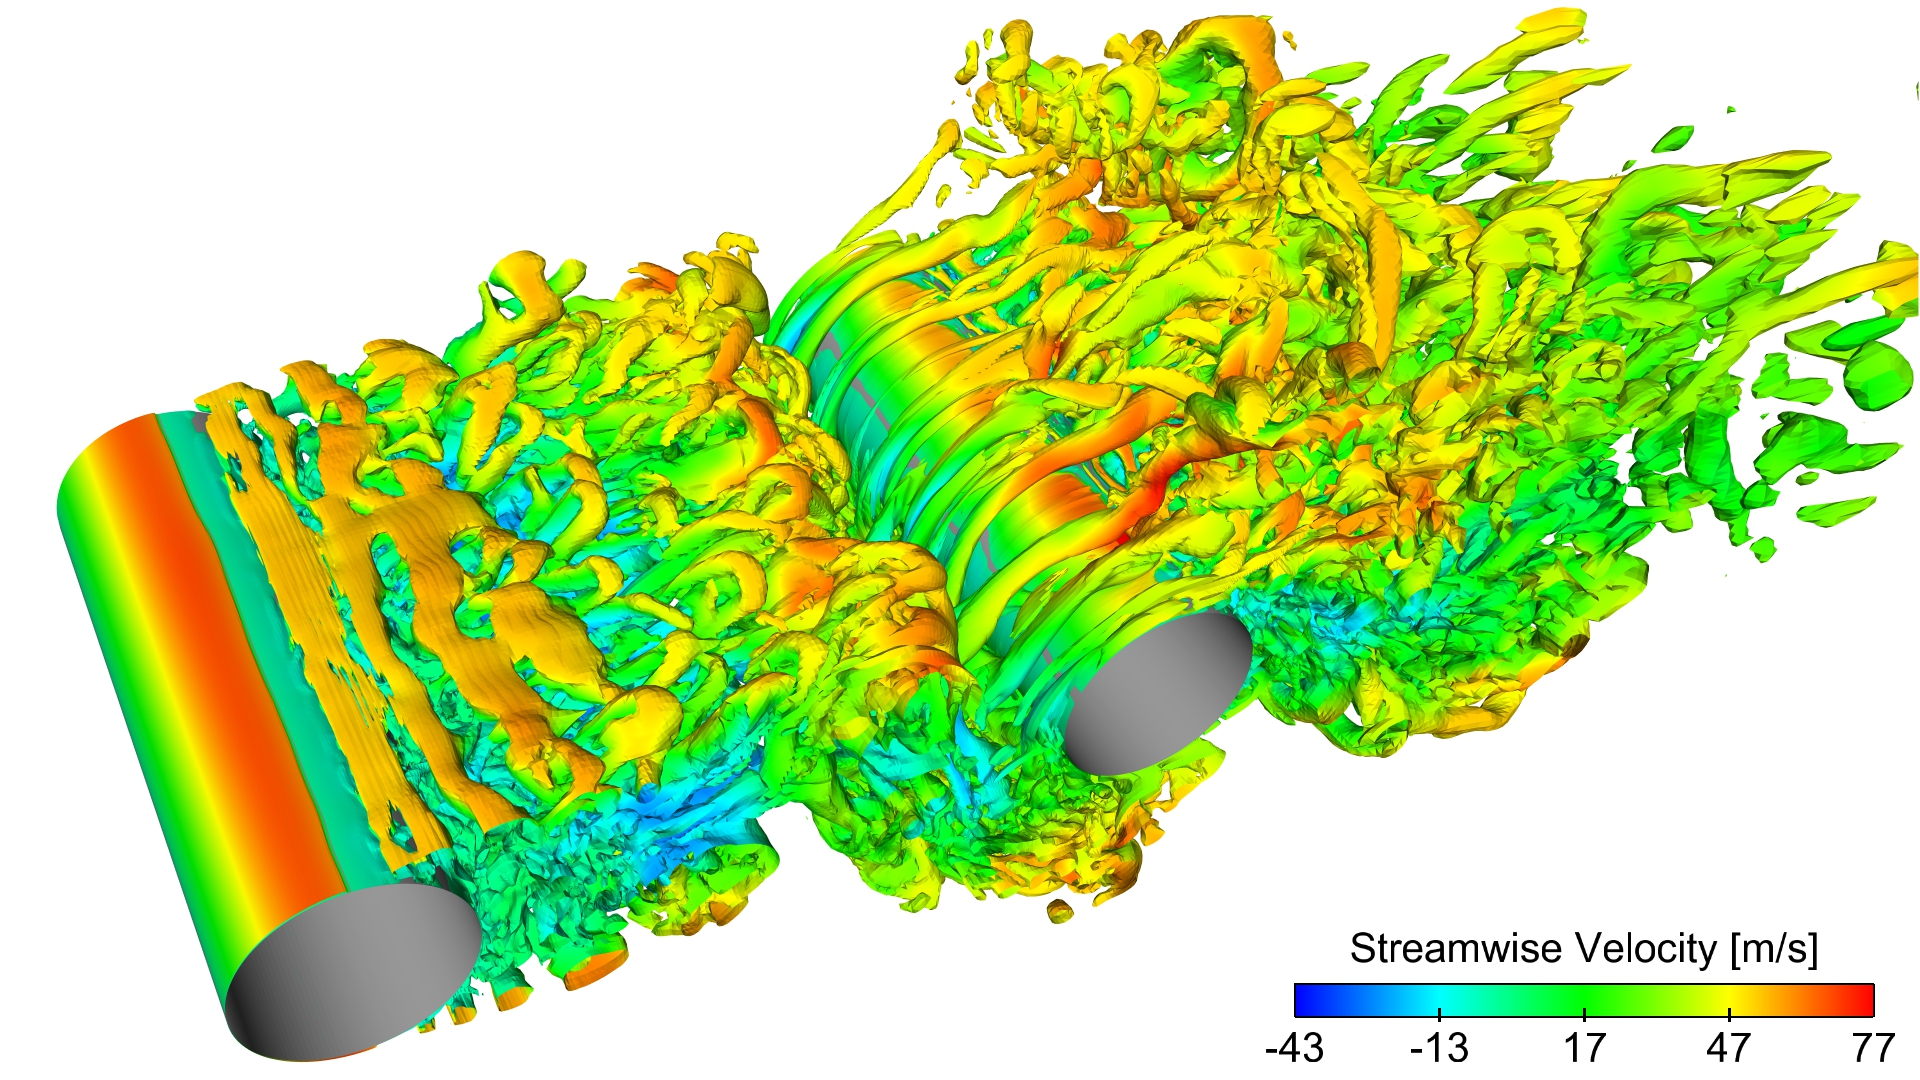
\includegraphics[width=0.40\textwidth]{tc_q_criteria}
    \bicaption{Q判据等值面图,同时测试一下一个很长的标题,比如这真的是一个很长很长很长很长很长很长很长很长的标题。}{Isocontour of Q criteria, at the same time, this is to test a long title, for instance, this is a really very long very long very long very long very long title.}
    \label{fig:tc_q_criteria}
\end{figure}

如果插图的空白区域过大,以图片\verb|shock_cyn|为例,自动裁剪如图\ref{fig:shock_cyn}。
\begin{figure}[!htbp]
    \centering
    %trim option's parameter order: left bottom right top
    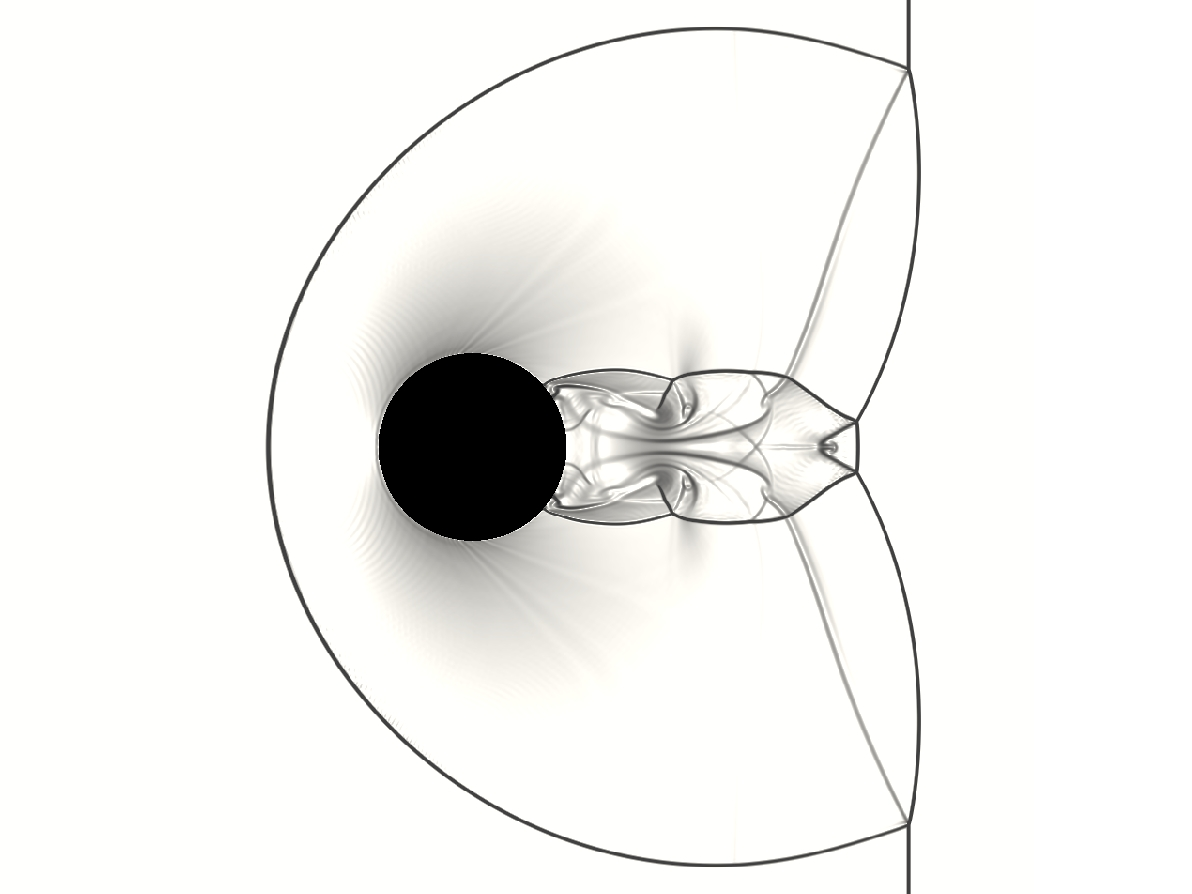
\includegraphics[trim = 30mm 0mm 30mm 0mm, clip, width=0.40\textwidth]{shock_cyn}
    \bicaption{激波圆柱作用。}{Shock-cylinder interaction.}
    \label{fig:shock_cyn}
\end{figure}

多图的插入如图\ref{fig:oaspl},多图不应在子图中给文本子标题,只要给序号,并在主标题中进行引用说明。
\begin{figure}[!htbp]
    \centering
    \begin{subfigure}[b]{0.35\textwidth}
      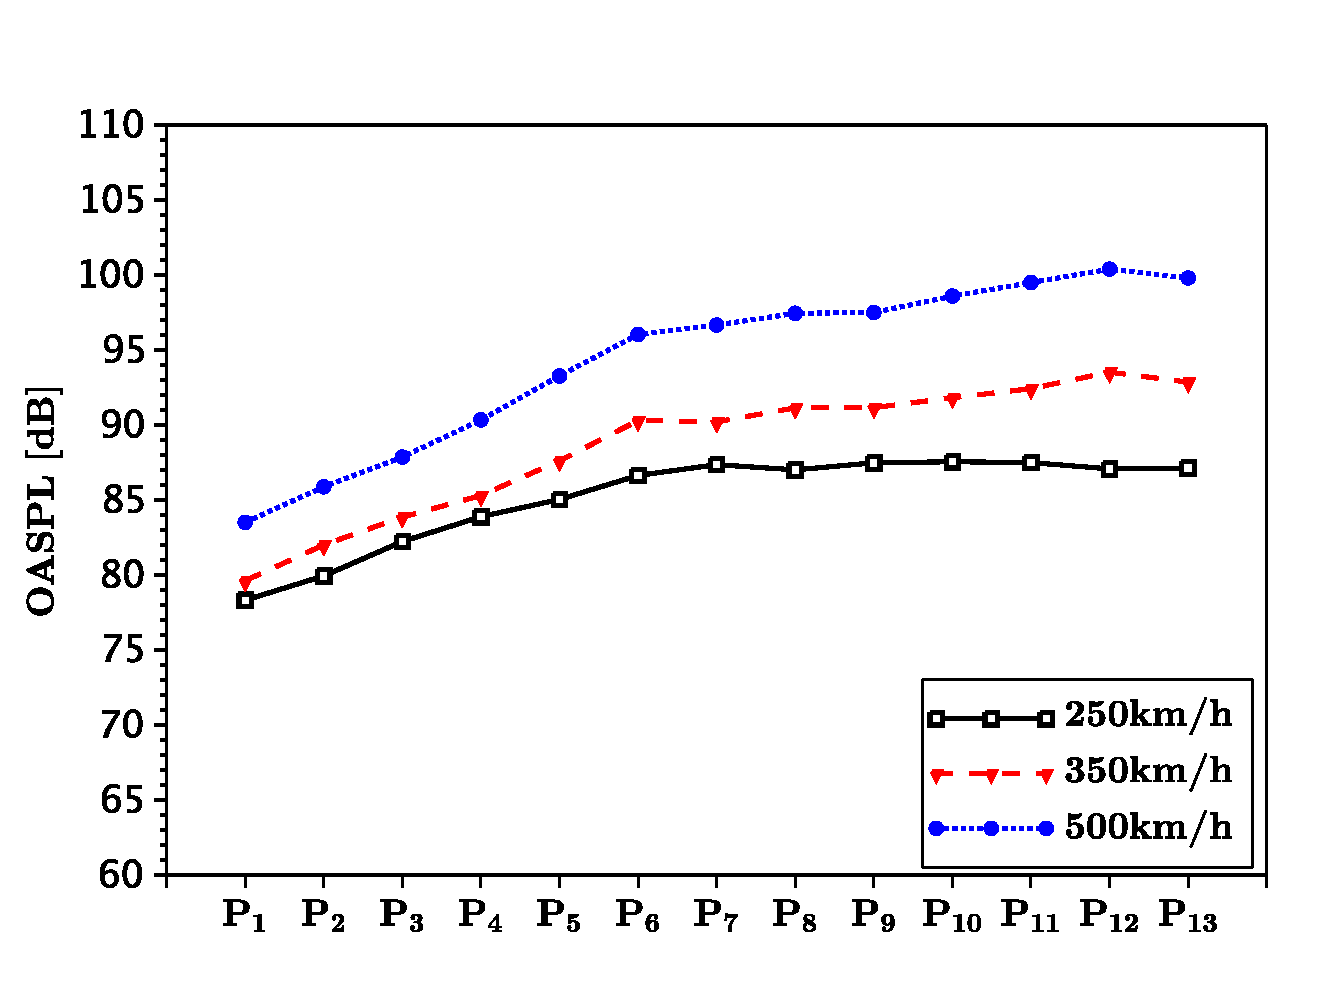
\includegraphics[width=\textwidth]{oaspl_a}
      \caption{}
      \label{fig:oaspl_a}
    \end{subfigure}%
    ~% add desired spacing
    \begin{subfigure}[b]{0.35\textwidth}
      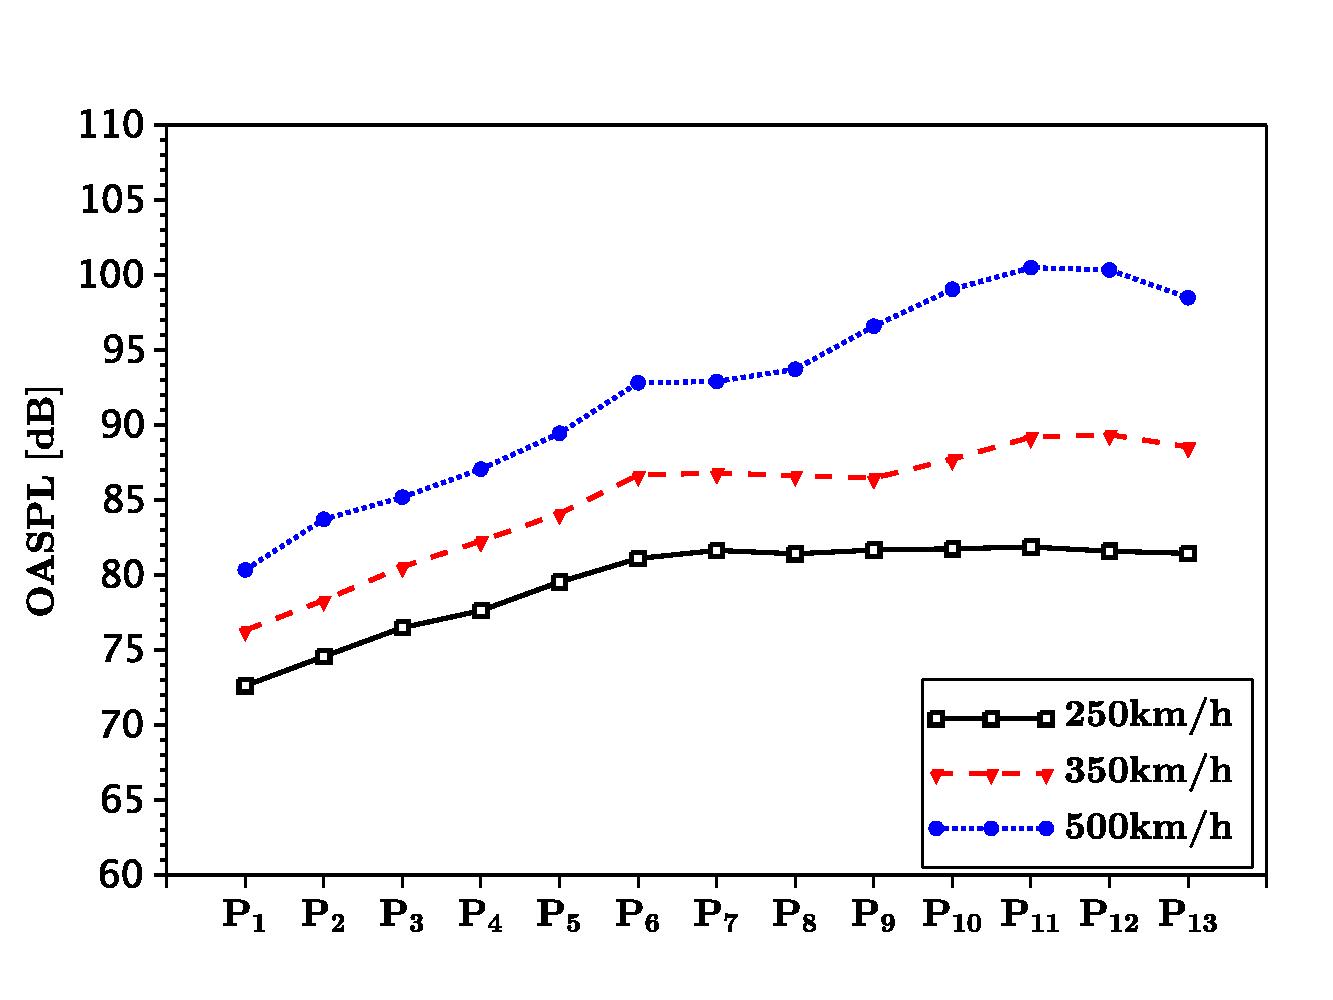
\includegraphics[width=\textwidth]{oaspl_b}
      \caption{}
      \label{fig:oaspl_b}
    \end{subfigure}
    \\% line break
    \begin{subfigure}[b]{0.35\textwidth}
      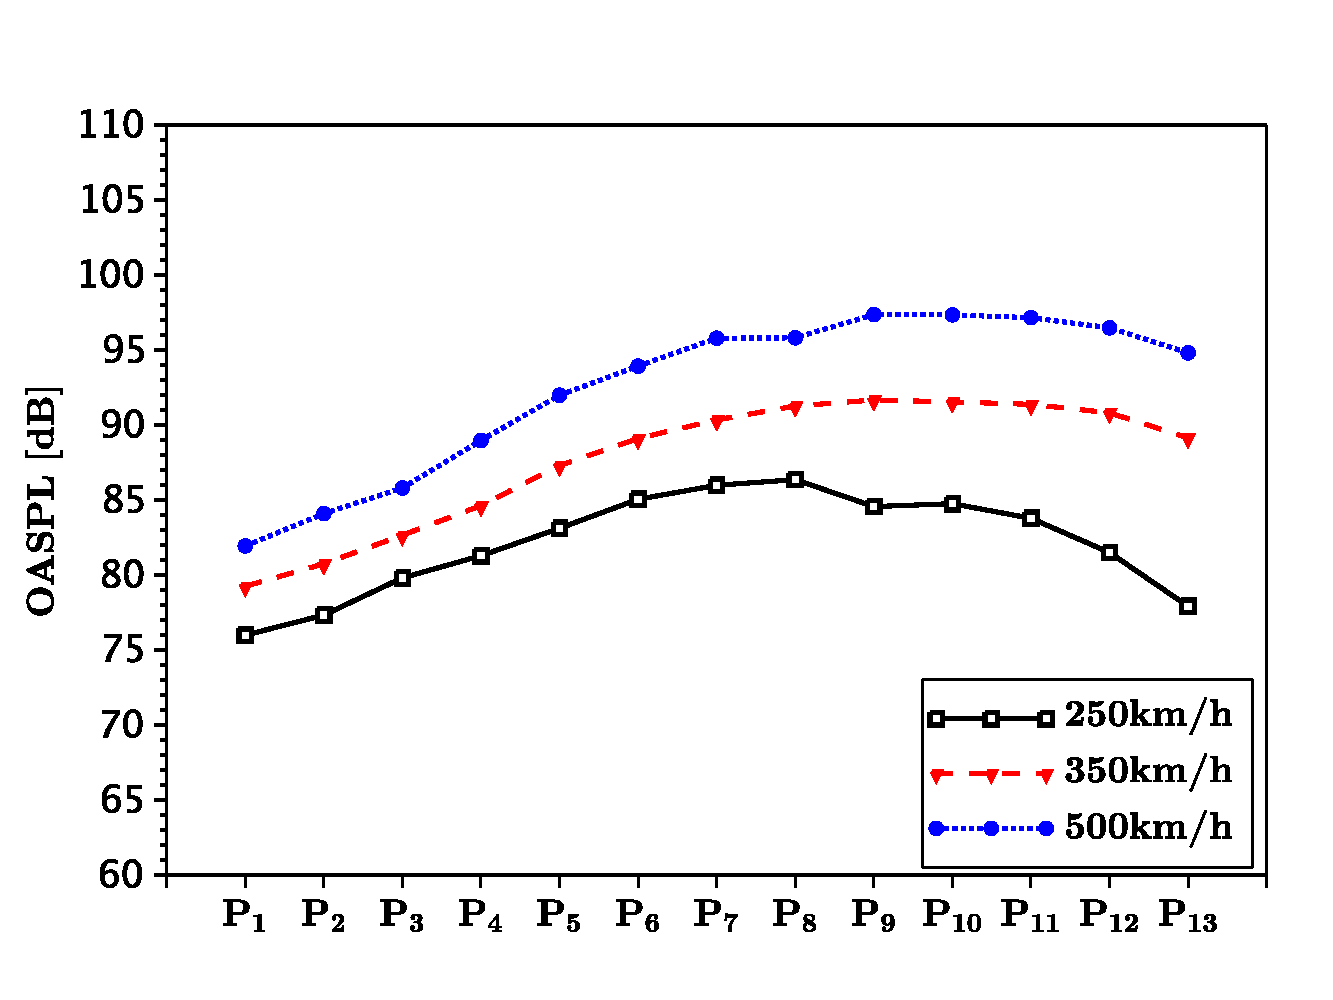
\includegraphics[width=\textwidth]{oaspl_c}
      \caption{}
      \label{fig:oaspl_c}
    \end{subfigure}%
    ~% add desired spacing
    \begin{subfigure}[b]{0.35\textwidth}
      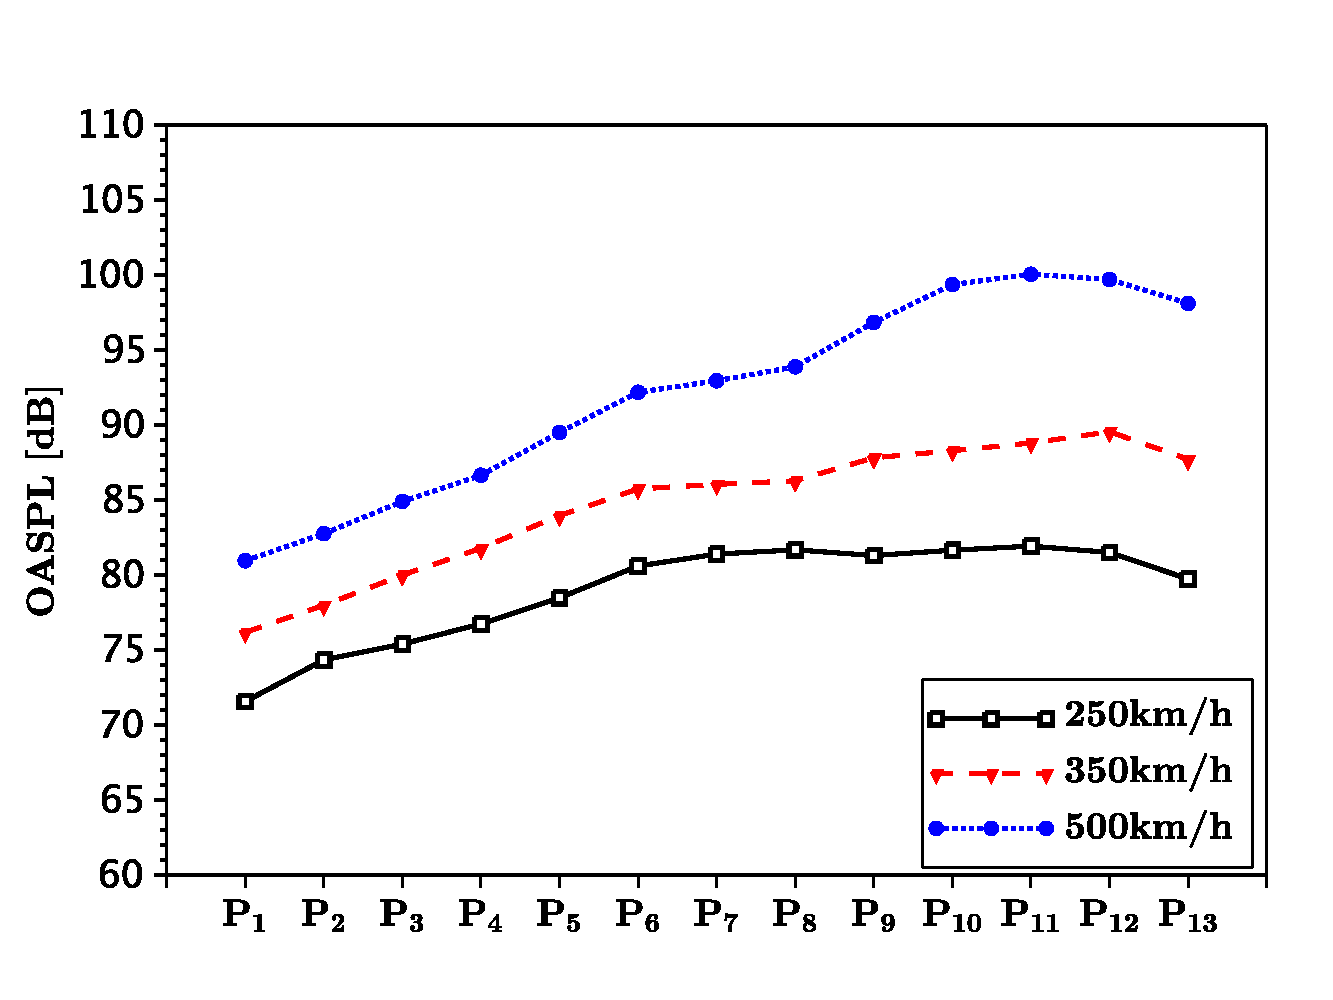
\includegraphics[width=\textwidth]{oaspl_d}
      \caption{}
      \label{fig:oaspl_d}
    \end{subfigure}
    \bicaption{总声压级。(a) 这是子图说明信息,(b) 这是子图说明信息,(c) 这是子图说明信息,(d) 这是子图说明信息。}{OASPL.(a) This is the explanation of subfig, (b) This is the explanation of subfig, (c) This is the explanation of subfig, (d) This is the explanation of subfig.}
    \label{fig:oaspl}
\end{figure}

\subsection{算法}

如见算法~\ref{alg:euclid},详细使用方法请参见文档 \href{https://ctan.org/pkg/algorithmicx?lang=en}{algorithmicx}。

\begin{algorithm}[!htbp]
    \small
    \caption{Euclid's algorithm}\label{alg:euclid}
    \begin{algorithmic}[1]
        \Procedure{Euclid}{$a,b$}\Comment{The g.c.d. of a and b}
        \State $r\gets a\bmod b$
        \While{$r\not=0$}\Comment{We have the answer if r is 0}
        \State $a\gets b$
        \State $b\gets r$
        \State $r\gets a\bmod b$
        \EndWhile\label{euclidendwhile}
        \State \textbf{return} $b$\Comment{The gcd is b}
        \EndProcedure
    \end{algorithmic}
\end{algorithm}

\subsection{参考文献引用}

参考文献引用过程以实例进行介绍,假设需要引用名为"Document Preparation System"的文献,步骤如下:

1)使用Google Scholar搜索Document Preparation System,在目标条目下点击Cite,展开后选择Import into BibTeX打开此文章的BibTeX索引信息,将它们copy添加到ref.bib文件中(此文件位于Biblio文件夹下)。

2)索引第一行 \verb|@article{lamport1986document,|中 \verb|lamport1986document| 即为此文献的label (\textbf{中文文献也必须使用英文label},一般遵照:姓氏拼音+年份+标题第一字拼音的格式),想要在论文中索引此文献,有两种索引类型:

文本类型:\verb|\citet{lamport1986document}|。正如此处所示 \citet{lamport1986document}; 

括号类型:\verb|\citep{lamport1986document}|。正如此处所示 \citep{lamport1986document}。

\textbf{多文献索引用英文逗号隔开}:

\verb|\citep{lamport1986document, chu2004tushu, chen2005zhulu}|。正如此处所示 \citep{lamport1986document, chu2004tushu, chen2005zhulu}

更多例子如:

\citet{walls2013drought} 根据 \citet{betts2005aging} 的研究,首次提出...。其中关于... \citep{walls2013drought, betts2005aging},是当前中国...得到迅速发展的研究领域 \citep{chen1980zhongguo, bravo1990comparative}。引用同一著者在同一年份出版的多篇文献时,在出版年份之后用
英文小写字母区别,如:\citep{yuan2012lana, yuan2012lanb, yuan2012lanc} 和 \citet{yuan2012lana, yuan2012lanb, yuan2012lanc}。同一处引用多篇文献时,按出版年份由近及远依次标注。例如 \citep{chen1980zhongguo, stamerjohanns2009mathml, hls2012jinji, niu2013zonghe}。

使用著者-出版年制(authoryear)式参考文献样式时,中文文献必须在BibTeX索引信息的 \textbf{key} 域(请参考ref.bib文件)填写作者姓名的拼音,才能使得文献列表按照拼音排序。参考文献表中的条目(不排序号),先按语种分类排列,语种顺 序是:中文、日文、英文、俄文、其他文种。然后,中文按汉语拼音字母顺序排列,日文按第一著者的姓氏笔画排序,西文和 俄文按第一著者姓氏首字母顺序排列。如中 \citep{niu2013zonghe}、日 \citep{Bohan1928}、英 \citep{stamerjohanns2009mathml}、俄 \citep{Dubrovin1906}。

如此,即完成了文献的索引,请查看下本文档的参考文献一章,看看是不是就是这么简单呢?是的,就是这么简单!

不同文献样式和引用样式,如著者-出版年制(authoryear)、顺序编码制(numbers)、上标顺序编码制(super)可在Thesis.tex中对artratex.sty调用实现,详见 \href{https://github.com/mohuangrui/ucasthesis/wiki}{ucasthesis 知识小站之文献样式}

%若在上标顺序编码制(super)模式下,希望在特定位置将上标改为嵌入式标,可使用 \citetns{niu2013zonghe,stamerjohanns2009mathml} 和 \citepns{niu2013zonghe,stamerjohanns2009mathml}。

参考文献索引的更多知识,请见 \href{https://en.wikibooks.org/wiki/LaTeX/Bibliography_Management}{WiKibook Bibliography}。\nocite{*}% 使文献列表显示所有参考文献(包括未引用文献)

\section{常见使用问题}\label{sec:qa}

\begin{enumerate}
    \item 模板每次发布前,都已在Windows,Linux,MacOS系统上测试通过。下载模板后,若编译出现错误,则请见 \href{https://github.com/mohuangrui/ucasthesis/wiki}{ucasthesis知识小站} 的 \href{https://github.com/mohuangrui/ucasthesis/wiki/%E7%BC%96%E8%AF%91%E6%8C%87%E5%8D%97}{编译指南}。

    \item 模板文档的编码为UTF-8编码。所有文件都必须采用UTF-8编码,否则编译后生成的文档将出现乱码文本。若出现文本编辑器无法打开文档或打开文档乱码的问题,请检查编辑器对UTF-8编码的支持。如果使用WinEdt作为文本编辑器(\textbf{不推荐使用}),应在其Options -> Preferences -> wrapping选项卡下将两种Wrapping Modes中的内容:
        
        TeX;HTML;ANSI;ASCII|DTX...
        
        修改为:TeX;\textbf{UTF-8|ACP;}HTML;ANSI;ASCII|DTX...
        
        同时,取消Options -> Preferences -> Unicode中的Enable ANSI Format。

    \item 推荐选择xelatex或lualatex编译引擎编译中文文档。编译脚本的默认设定为xelatex编译引擎。你也可以选择不使用脚本编译,如直接使用 \LaTeX{}文本编辑器编译。注:\LaTeX{}文本编辑器编译的默认设定为pdflatex编译引擎,若选择xelatex或lualatex编译引擎,请进入下拉菜单选择。为正确生成引用链接和参考文献,需要进行\textbf{全编译}。

    \item Texmaker使用简介
        \begin{enumerate}
            \footnotesize
            \item 使用 Texmaker “打开 (Open)” Thesis.tex。
            \item 菜单 “选项 (Options)” -> “设置当前文档为主文档 (Define as Master Document)”
            \item 菜单 “自定义 (User)” -> “自定义命令 (User Commands)” -> “编辑自定义命令 (Edit User Commands)” -> 左侧选择 “command 1”,右侧 “菜单项 (Menu Item)” 填入 Auto Build -> 点击下方“向导 (Wizard)” -> “添加 (Add)”: xelatex + bibtex + xelatex + xelatex + pdf viewer -> 点击“完成 (OK)”
            \item 使用 Auto Build 编译带有未生成引用链接的源文件,可以仅使用 xelatex 编译带有已经正确生成引用链接的源文件。
            \item 编译完成,“查看(View)” PDF,在PDF中 “ctrl+click” 可链接到相对应的源文件。
        \end{enumerate}
    
    \item 模版的设计可能地考虑了适应性。致谢等所有条目都是通过最为通用的

        \verb+\chapter{item name}+  and \verb+\section*{item name}+

        来显式实现的 (请观察Backmatter.tex),从而可以随意添加,放置,和修改,如同一般章节。对于图表目录名称则可在ucasthesis.cfg中进行修改。

    \item 设置文档样式: 在artratex.sty中搜索关键字定位相应命令,然后修改
        \begin{enumerate}
            \item 正文行距:启用和设置 \verb|\linespread{1.5}|,默认1.5倍行距。
            \item 参考文献行距:修改 \verb|\setlength{\bibsep}{0.0ex}|
            \item 目录显示级数:修改 \verb|\setcounter{tocdepth}{2}|
            \item 文档超链接的颜色及其显示:修改 \verb|\hypersetup|
        \end{enumerate}

    \item 文档内字体切换方法:
        \begin{itemize}
            \item 宋体:国科大论文模板ucasthesis 或 \textrm{国科大论文模板ucasthesis}
            \item 粗宋体:{\bfseries 国科大论文模板ucasthesis} 或 \textbf{国科大论文模板ucasthesis}
            \item 黑体:{\sffamily 国科大论文模板ucasthesis} 或 \textsf{国科大论文模板ucasthesis}
            \item 粗黑体:{\bfseries\sffamily 国科大论文模板ucasthesis} 或 \textsf{\bfseries 国科大论文模板ucasthesis}
            \item 仿宋:{\ttfamily 国科大论文模板ucasthesis} 或 \texttt{国科大论文模板ucasthesis}
            \item 粗仿宋:{\bfseries\ttfamily 国科大论文模板ucasthesis} 或 \texttt{\bfseries 国科大论文模板ucasthesis}
            \item 楷体:{\itshape 国科大论文模板ucasthesis} 或 \textit{国科大论文模板ucasthesis}
            \item 粗楷体:{\bfseries\itshape 国科大论文模板ucasthesis} 或 \textit{\bfseries 国科大论文模板ucasthesis}
        \end{itemize}
\end{enumerate}



%---------------------------------------------------------------------------%
% main content
%-
%-> Appendix
%-
\cleardoublepage%
\appendix% initialize the environment
\chapter{第一个程序}\label{apdx:第一个程序}
\section{主核}
\begin{lstlisting}
#include <stdlib.h>
#include <stdio.h>
#include <athread.h>
#include <sys/time.h>
#include <sys/types.h>
#include <sys/stat.h>
#include <fcntl.h>

extern SLAVE_FUN(func)();

#define X 64
#define Y 2048

int A[X][Y], B[X][Y], C[X][Y],CC[X][Y];

void init()
{
    int i, j;
    for (i = 0; i < X; i++)
        for (j = 0; j < Y; j++)
        {
            A[i][j] = i + j;
            B[i][j] = i + j + 1;
            C[i][j] = 0;
            CC[i][j]=0;
        }
    printf("Init finished\n");
}

int main(void)
{
    int i, j;
    struct timeval start, end;
    init();
    double time_use;
    printf("No boost proceed:\n");
    gettimeofday(&start, NULL);
    for (i = 0; i < X; i++)
        for (j = 0; j < Y; j++)
            C[i][j] = A[i][j] + B[i][j];
    gettimeofday(&end, NULL);
    time_use = 1000000 * (end.tv_sec - start.tv_sec) + end.tv_usec - start.tv_usec;
    printf("Time usage is %lf us\n", time_use);
    printf("(C[32][0], C[63][999]) = (%d, %d)\n", C[32][0], C[63][999]);
    init();
    athread_init();
    printf("Boosted proceed:\n");
    gettimeofday(&start, NULL);
    athread_spawn(func, 0);
    athread_join();
    gettimeofday(&end, NULL);
    time_use = 1000000 * (end.tv_sec - start.tv_sec) + end.tv_usec - start.tv_usec;
    printf("Time usage is %lf us\n", time_use);
    printf("(C[32][0], C[63][999]) = (%d, %d)\n", C[32][0], C[63][999]);
    athread_halt();
    return 0;
}
\end{lstlisting}

\section{从核}
\begin{lstlisting}
#include <stdio.h>
#include <math.h>
#include <string.h>
#include "slave.h"
#define X 64
#define Y 2048

#define Y0 64
#define N 32
//Y0*N=Y

#define L0 256
//L0=Y*4

__thread_local int my_id;
__thread_local volatile unsigned long get_reply[N], put_reply = 0;
extern int A[X][Y], B[X][Y], C[X][Y], CC[X][Y];

__thread_local int A_slave[Y], B_slave[Y], C_slave[Y];

void func()
{
	int i, j, t,tt;
	put_reply=0;
	my_id = athread_get_id(-1);

	for (i = 0; i < N; i++)//输入数据
	{
		get_reply[i]=0;
		t = i * Y0; //当前位置
		athread_get(PE_MODE, &A[my_id][t], &A_slave[t], L0,
		 &get_reply[i], 0, 0, 0);
		athread_get(PE_MODE, &B[my_id][t], &B_slave[t], L0,
		 &get_reply[i], 0, 0, 0);
	}

	for (i = 0; i < N; i++)//计算
	{
		t = i * Y0; //当前起始位置
		while (get_reply[i] != 2);
		for (j = 0; j < Y0; j++)
		{
			tt=t+j;
			C_slave[tt] = A_slave[tt] + B_slave[tt];
		}
		athread_put(PE_MODE, &C_slave[t], &C[my_id][t], L0, &put_reply, 0, 0);
	}
	while (put_reply != N);
}
\end{lstlisting}

\chapter{Darknet的Makefile}\label{apdx:Darknet的Makefile}
\begin{lstlisting}[language=make]
GPU=0
CUDNN=0
OPENCV=0
OPENMP=0
DEBUG=0

ARCH= -gencode arch=compute_30,code=sm_30 \
        -gencode arch=compute_35,code=sm_35 \
        -gencode arch=compute_50,code=[sm_50,compute_50] \
        -gencode arch=compute_52,code=[sm_52,compute_52]
#      -gencode arch=compute_20,code=[sm_20,sm_21] \ This one is deprecated?

# This is what I use, uncomment if you know your arch and want to specify
# ARCH= -gencode arch=compute_52,code=compute_52

VPATH=./src/:./examples
SLIB=libdarknet.so
ALIB=libdarknet.a
EXEC=darknet
OBJDIR=./obj/

CC=gcc
CPP=g++
NVCC=nvcc 
AR=ar
ARFLAGS=rcs
OPTS=-Ofast
LDFLAGS= -lm -pthread 
COMMON= -Iinclude/ -Isrc/
CFLAGS=-Wall -Wno-unused-result -Wno-unknown-pragmas -Wfatal-errors -fPIC

ifeq ($(OPENMP), 1) 
CFLAGS+= -fopenmp
endif

ifeq ($(DEBUG), 1) 
OPTS=-O0 -g
endif

CFLAGS+=$(OPTS)

ifeq ($(OPENCV), 1) 
COMMON+= -DOPENCV
CFLAGS+= -DOPENCV
LDFLAGS+= `pkg-config --libs opencv` -lstdc++
COMMON+= `pkg-config --cflags opencv` 
endif

ifeq ($(GPU), 1) 
COMMON+= -DGPU -I/usr/local/cuda/include/
CFLAGS+= -DGPU
LDFLAGS+= -L/usr/local/cuda/lib64 -lcuda -lcudart -lcublas -lcurand
endif

ifeq ($(CUDNN), 1) 
COMMON+= -DCUDNN 
CFLAGS+= -DCUDNN
LDFLAGS+= -lcudnn
endif

OBJ=gemm.o utils.o cuda.o deconvolutional_layer.o convolutional_layer.o list.o image.o activations.o im2col.o col2im.o blas.o crop_layer.o dropout_layer.o maxpool_layer.o softmax_layer.o data.o matrix.o network.o connected_layer.o cost_layer.o parser.o option_list.o detection_layer.o route_layer.o upsample_layer.o box.o normalization_layer.o avgpool_layer.o layer.o local_layer.o shortcut_layer.o logistic_layer.o activation_layer.o rnn_layer.o gru_layer.o crnn_layer.o demo.o batchnorm_layer.o region_layer.o reorg_layer.o tree.o  lstm_layer.o l2norm_layer.o yolo_layer.o iseg_layer.o image_opencv.o
EXECOBJA=captcha.o lsd.o super.o art.o tag.o cifar.o go.o rnn.o segmenter.o regressor.o classifier.o coco.o yolo.o detector.o nightmare.o instance-segmenter.o darknet.o
ifeq ($(GPU), 1) 
LDFLAGS+= -lstdc++ 
OBJ+=convolutional_kernels.o deconvolutional_kernels.o activation_kernels.o im2col_kernels.o col2im_kernels.o blas_kernels.o crop_layer_kernels.o dropout_layer_kernels.o maxpool_layer_kernels.o avgpool_layer_kernels.o
endif

EXECOBJ = $(addprefix $(OBJDIR), $(EXECOBJA))
OBJS = $(addprefix $(OBJDIR), $(OBJ))
DEPS = $(wildcard src/*.h) Makefile include/darknet.h

all: obj backup results $(SLIB) $(ALIB) $(EXEC)
#all: obj  results $(SLIB) $(ALIB) $(EXEC)


$(EXEC): $(EXECOBJ) $(ALIB)
    $(CC) $(COMMON) $(CFLAGS) $^ -o $@ $(LDFLAGS) $(ALIB)

$(ALIB): $(OBJS)
    $(AR) $(ARFLAGS) $@ $^

$(SLIB): $(OBJS)
    $(CC) $(CFLAGS) -shared $^ -o $@ $(LDFLAGS)

$(OBJDIR)%.o: %.cpp $(DEPS)
    $(CPP) $(COMMON) $(CFLAGS) -c $< -o $@

$(OBJDIR)%.o: %.c $(DEPS)
    $(CC) $(COMMON) $(CFLAGS) -c $< -o $@

$(OBJDIR)%.o: %.cu $(DEPS)
    $(NVCC) $(ARCH) $(COMMON) --compiler-options "$(CFLAGS)" -c $< -o $@

obj:
    mkdir -p obj
backup:
    mkdir -p backup
results:
    mkdir -p results

.PHONY: clean

clean:
    rm -rf $(OBJS) $(SLIB) $(ALIB) $(EXEC) $(EXECOBJ) $(OBJDIR)/*    
\end{lstlisting}
\chapter{中国科学院大学学位论文撰写要求}

学位论文是研究生科研工作成果的集中体现,是评判学位申请者学术水平、授予其学位的主要依据,是科研领域重要的文献资料。根据《科学技术报告、学位论文和学术论文的编写格式》(GB/T 7713-1987)、《学位论文编写规则》(GB/T 7713.1-2006)和《文后参考文献著录规则》(GB7714—87)等国家有关标准,结合中国科学院大学(以下简称“国科大”)的实际情况,特制订本规定。

\section{论文无附录者无需附录部分}

\section{测试公式编号 \texorpdfstring{$\Lambda,\lambda,\theta,\bar{\Lambda},\sqrt{S_{NN}}$}{$\textLambda,\textlambda,\texttheta,\bar{\textLambda},\sqrt{S_{NN}}$}} \label{sec:testmath}

\begin{equation} \label{eq:appedns}
    \adddotsbeforeeqnnum%
    \begin{cases}
        \frac{\partial \rho}{\partial t} + \nabla\cdot(\rho\Vector{V}) = 0\\
        \frac{\partial (\rho\Vector{V})}{\partial t} + \nabla\cdot(\rho\Vector{V}\Vector{V}) = \nabla\cdot\Tensor{\sigma}\\
        \frac{\partial (\rho E)}{\partial t} + \nabla\cdot(\rho E\Vector{V}) = \nabla\cdot(k\nabla T) + \nabla\cdot(\Tensor{\sigma}\cdot\Vector{V})
    \end{cases}
\end{equation}
\begin{equation}
    \adddotsbeforeeqnnum%
    \frac{\partial }{\partial t}\int\limits_{\Omega} u \, \mathrm{d}\Omega + \int\limits_{S} \unitVector{n}\cdot(u\Vector{V}) \, \mathrm{d}S = \dot{\phi}
\end{equation}
\[
    \begin{split}
        \mathcal{L} \{f\}(s) &= \int _{0^{-}}^{\infty} f(t) e^{-st} \, \mathrm{d}t, \ 
        \mathscr{L} \{f\}(s) = \int _{0^{-}}^{\infty} f(t) e^{-st} \, \mathrm{d}t\\
        \mathcal{F} {\bigl (} f(x+x_{0}) {\bigr )} &= \mathcal{F} {\bigl (} f(x) {\bigr )} e^{2\pi i\xi x_{0}}, \ 
        \mathscr{F} {\bigl (} f(x+x_{0}) {\bigr )} = \mathscr{F} {\bigl (} f(x) {\bigr )} e^{2\pi i\xi x_{0}}
    \end{split}
\]

mathtext: $A,F,L,2,3,5,\sigma$, mathnormal: $A,F,L,2,3,5,\sigma$, mathrm: $\mathrm{A,F,L,2,3,5,\sigma}$.

mathbf: $\mathbf{A,F,L,2,3,5,\sigma}$, mathit: $\mathit{A,F,L,2,3,5,\sigma}$, mathsf: $\mathsf{A,F,L,2,3,5,\sigma}$.

mathtt: $\mathtt{A,F,L,2,3,5,\sigma}$, mathfrak: $\mathfrak{A,F,L,2,3,5,\sigma}$, mathbb: $\mathbb{A,F,L,2,3,5,\sigma}$.

mathcal: $\mathcal{A,F,L,2,3,5,\sigma}$, mathscr: $\mathscr{A,F,L,2,3,5,\sigma}$, boldsymbol: $\boldsymbol{A,F,L,2,3,5,\sigma}$.

vector: $\Vector{\sigma, T, a, F, n}$, unitvector: $\unitVector{\sigma, T, a, F, n}$

matrix: $\Matrix{\sigma, T, a, F, n}$, unitmatrix: $\unitMatrix{\sigma, T, a, F, n}$

tensor: $\Tensor{\sigma, T, a, F, n}$, unittensor: $\unitTensor{\sigma, T, a, F, n}$ 

\section{测试生僻字}

霜蟾盥薇曜灵霜颸妙鬘虚霩淩澌菀枯菡萏泬寥窅冥毰毸濩落霅霅便嬛岧峣瀺灂姽婳愔嫕飒纚棽俪緸冤莩甲摛藻卮言倥侗椒觞期颐夜阑彬蔚倥偬澄廓簪缨陟遐迤逦缥缃鹣鲽憯懔闺闼璀错媕婀噌吰澒洞阛闠覼缕玓瓑逡巡諓諓琭琭瀌瀌踽踽叆叇氤氲瓠犀流眄蹀躞赟嬛茕頔璎珞螓首蘅皋惏悷缱绻昶皴皱颟顸愀然菡萏卑陬纯懿犇麤掱暒 墌墍墎墏墐墒墒墓墔墕墖墘墖墚墛坠墝增墠墡墢墣墤墥墦墧墨墩墪樽墬墭堕墯墰墱墲坟墴墵垯墷墸墹墺墙墼墽垦墿壀壁壂壃壄壅壆坛壈壉壊垱壌壍埙壏壐壑壒压壔壕壖壗垒圹垆壛壜壝垄壠壡坜壣壤壥壦壧壨坝塆圭嫶嫷嫸嫹嫺娴嫼嫽嫾婳妫嬁嬂嬃嬄嬅嬆嬇娆嬉嬊娇嬍嬎嬏嬐嬑嬒嬓嬔嬕嬖嬗嬘嫱嬚嬛嬜嬞嬟嬠嫒嬢嬣嬥嬦嬧嬨嬩嫔嬫嬬奶嬬嬮嬯婴嬱嬲嬳嬴嬵嬶嬷婶嬹嬺嬻嬼嬽嬾嬿孀孁孂娘孄孅孆孇孆孈孉孊娈孋孊孍孎孏嫫婿媚嵭嵮嵯嵰嵱嵲嵳嵴嵵嵶嵷嵸嵹嵺嵻嵼嵽嵾嵿嶀嵝嶂嶃崭嶅嶆岖嶈嶉嶊嶋嶌嶍嶎嶏嶐嶑嶒嶓嵚嶕嶖嶘嶙嶚嶛嶜嶝嶞嶟峤嶡峣嶣嶤嶥嶦峄峃嶩嶪嶫嶬嶭崄嶯嶰嶱嶲嶳岙嶵嶶嶷嵘嶹岭嶻屿岳帋巀巁巂巃巄巅巆巇巈巉巊岿巌巍巎巏巐巑峦巓巅巕岩巗巘巙巚帠帡帢帣帤帨帩帪帬帯帰帱帲帴帵帷帹帺帻帼帽帾帿幁幂帏幄幅幆幇幈幉幊幋幌幍幎幏幐幑幒幓幖幙幚幛幜幝幞帜幠幡幢幤幥幦幧幨幩幪幭幮幯幰幱庍庎庑庖庘庛庝庠庡庢庣庤庥庨庩庪庬庮庯庰庱庲庳庴庵庹庺庻庼庽庿廀厕廃厩廅廆廇廋廌廍庼廏廐廑廒廔廕廖廗廘廙廛廜廞庑廤廥廦廧廨廭廮廯廰痈廲廵廸廹廻廼廽廿弁弅弆弇弉弖弙弚弜弝弞弡弢弣弤弨弩弪弫弬弭弮弰弲弪弴弶弸弻弼弽弿彖彗彘彚彛彜彝彞彟彴彵彶彷彸役彺彻彽彾佛徂徃徆徇徉后徍徎徏径徒従徔徕徖徙徚徛徜徝从徟徕御徢徣徤徥徦徧徨复循徫旁徭微徯徰徱徲徳徴徵徶德徸彻徺忁忂惔愔忇忈忉忔忕忖忚忛応忝忞忟忪挣挦挧挨挩挪挫挬挭挮挰掇授掉掊掋掍掎掐掑排掓掔掕挜掚挂掜掝掞掟掠采探掣掤掦措掫掬掭掮掯掰掱掲掳掴掵掶掸掹掺掻掼掽掾掿拣揁揂揃揅揄揆揇揈揉揊揋揌揍揎揑揓揔揕揖揗揘揙揤揥揦揧揨揫捂揰揱揲揳援揵揶揷揸揻揼揾揿搀搁搂搃搄搅搇搈搉搊搋搌搎搏搐搑搒摓摔摕摖摗摙摚摛掼摝摞摠摡斫斩斮斱斲斳斴斵斶斸旪旫旮旯晒晓晔晕晖晗晘晙晛晜晞晟晠晡晰晣晤晥晦晧晪晫晬晭晰晱晲晳晴晵晷晸晹晻晼晽晾晿暀暁暂暃暄暅暆暇晕晖暊暋暌暍暎暏暐暑暒暓暔暕暖暗旸暙暚暛暜暝暞暟暠暡暣暤暥暦暧暨暩暪暬暭暮暯暰昵暲暳暴暵暶暷暸暹暺暻暼暽暾暿曀曁曂曃晔曅曈曊曋曌曍曎曏曐曑曒曓曔曕曗曘曙曚曛曜曝曞曟旷曡曢曣曤曥曦曧昽曩曪曫晒曭曮曯椗椘椙椚椛検椝椞椟椠椡椢椣椤椥椦椧椨椩椪椫椬椭椮。
% appendix content
%-
%-> Backmatter: bibliography, glossary, index
%-
\backmatter% initialize the environment
\intotoc*{\cleardoublepage}{\bibname}% add link to toc
\bibliography{Biblio/ref}% bibliography
{% content list region
\linespread{1.2}% local line space
\intotoc*{\cleardoublepage}{\listfigurename}% add link to bookmark
\listoffigures% figure catalog
\intotoc*{\cleardoublepage}{\listtablename}% add link to bookmark
\listoftables% table catalog
}
%---------------------------------------------------------------------------%
%->> Backmatter
%---------------------------------------------------------------------------%
\chapter{作者简历及攻读学位期间发表的学术论文与研究成果}

\textbf{本科生无需此部分}。

\section*{作者简历}

\subsection*{casthesis作者}

吴凌云,福建省屏南县人,中国科学院数学与系统科学研究院博士研究生。

\subsection*{ucasthesis作者}

莫晃锐,湖南省湘潭县人,中国科学院力学研究所硕士研究生。

\section*{已发表(或正式接受)的学术论文:}

[1] ucasthesis: A LaTeX Thesis Template for the University of Chinese Academy of Sciences, 2014.

\section*{申请或已获得的专利:}

(无专利时此项不必列出)

\section*{参加的研究项目及获奖情况:}

可以随意添加新的条目或是结构。

\chapter[致谢]{致\quad 谢}\chaptermark{致\quad 谢}% syntax: \chapter[目录]{标题}\chaptermark{页眉}
\thispagestyle{noheaderstyle}% 如果需要移除当前页的页眉
%\pagestyle{noheaderstyle}% 如果需要移除整章的页眉

感激casthesis作者吴凌云学长,gbt7714-bibtex-style
开发者zepinglee,和ctex众多开发者们。若没有他们的辛勤付出和非凡工作,\LaTeX{}菜鸟的我是无法完成此国科大学位论文\LaTeX{}模板ucasthesis的。在\LaTeX{}中的一点一滴的成长源于开源社区的众多优秀资料和教程,在此对所有\LaTeX{}社区的贡献者表示感谢!

ucasthesis国科大学位论文\LaTeX{}模板的最终成型离不开以霍明虹老师和丁云云老师为代表的国科大学位办公室老师们制定的官方指导文件和众多ucasthesis用户的热心测试和耐心反馈,在此对他们的认真付出表示感谢。特别对国科大的赵永明同学的众多有效反馈意见和建议表示感谢,对国科大本科部的陆晴老师和本科部学位办的丁云云老师的细致审核和建议表示感谢。谢谢大家的共同努力和支持,让ucasthesis为国科大学子使用\LaTeX{}撰写学位论文提供便利和高效这一目标成为可能。

\cleardoublepage[plain]% 让文档总是结束于偶数页,可根据需要设定页眉页脚样式,如 [noheaderstyle]
%---------------------------------------------------------------------------%
% other information
\end{document}
%---------------------------------------------------------------------------%

